\documentclass[12pt,a4paper]{report}

\usepackage[utf8]{inputenc}
\usepackage[T1]{fontenc}
\usepackage[french]{babel}

\usepackage[a4paper,margin=2.5cm]{geometry}
\usepackage{setspace}
\onehalfspacing
\usepackage{parskip}
\usepackage{textcomp}

\setlength{\parskip}{0.6em}
\setlength{\parindent}{0pt}

\widowpenalty=10000
\clubpenalty=10000
\displaywidowpenalty=10000

\usepackage[hidelinks]{hyperref}
\usepackage{bookmark}

\usepackage{graphicx}
\usepackage{float}
\usepackage{caption}
\usepackage{subcaption}
\usepackage{booktabs}
\usepackage{array}
\usepackage{longtable}
\usepackage{multirow}
\usepackage{colortbl}   % AJOUTÉ pour couleur dans Gantt
\usepackage{pgfgantt}   % AJOUTÉ pour diagramme de Gantt
\usepackage{needspace}

\usepackage{listings}
\usepackage{xcolor}
\usepackage{amsmath}
\usepackage{amssymb}
\usepackage{enumitem}

\definecolor{codebg}{RGB}{245,245,245}
\definecolor{codekw}{RGB}{0,92,197}
\definecolor{codecm}{RGB}{0,128,0}
\definecolor{codestr}{RGB}{163,21,21}

\lstdefinestyle{nexora}{
  backgroundcolor=\color{codebg},
  basicstyle=\ttfamily\small,
  keywordstyle=\color{codekw}\bfseries,
  commentstyle=\color{codecm},
  stringstyle=\color{codestr},
  numbers=left,
  numberstyle=\tiny,
  stepnumber=1,
  numbersep=8pt,
  frame=single,
  breaklines=true,
  showstringspaces=false,
  tabsize=2
}
\lstset{style=nexora}

\lstdefinelanguage{json}{
  keywords={false,true,null},
  keywordstyle=\color{codekw}\bfseries,
  sensitive=false,
  comment=[l]{//},
  morecomment=[s]{/*}{*/},
  commentstyle=\color{codecm},
  string=[b]",
  stringstyle=\color{codestr},
}

\title{NEXORA --- Plateforme d'Intelligence Organisationnelle}
\author{Soubaibi Omar \and Yassine Baizi}
\date{Année Universitaire 2025--2026}

\newcommand{\figref}[1]{Figure~\ref{#1}}
\newcommand{\tabref}[1]{Tableau~\ref{#1}}

\begin{document}

% =========================================================
% PAGE DE GARDE
% =========================================================
\begin{titlepage}
  \begin{center}
    
\includegraphics[width=0.22\textwidth]{emsilogo.jpeg}\par\vspace{0.8cm}

    {\Large EMSI --- École Marocaine des Sciences de l'Ingénieur (Casablanca)\par}
    \vspace{0.4cm}
    {\Large \textbf{Rapport de Projet de Fin d'Année}\par}
    \vspace{1.4cm}

    {\Huge \textbf{NEXORA}\par}
    \vspace{0.3cm}
    {\Large Plateforme d'Intelligence Organisationnelle\par}

    \vspace{1.6cm}

    \begin{tabular}{rl}
      \textbf{Réalisé par :} & Soubaibi Omar \\
      & Yassine Baizi \\
      \textbf{Encadré par :} & Mme. Ounacer Soumaya \\
      \textbf{Filière :} & 4IADM G5-A \\
      \textbf{Année Universitaire :} & 2025--2026 \\
    \end{tabular}

    \vfill
  \end{center}
\end{titlepage}

\clearpage

\pagenumbering{roman}

% =========================================================
% DÉDICACE
% =========================================================
\newpage
\chapter*{Dédicace}
\addcontentsline{toc}{chapter}{Dédicace}

Nous dédions ce travail à nos familles, dont le soutien constant, la patience et les encouragements ont constitué un socle indispensable tout au long de ce projet. Leur confiance nous a permis de maintenir l'exigence et la persévérance nécessaires à la réalisation d'un système ambitieux, à la croisée de l'intelligence artificielle, du Big Data et de l'ingénierie logicielle.

Nous dédions également ce rapport à toutes les personnes qui, de près ou de loin, ont contribué à l'aboutissement de NEXORA, que ce soit par un conseil, une relecture, un retour critique ou un soutien moral. Chaque interaction a participé à renforcer la rigueur de la démarche et la qualité du résultat.

Enfin, nous dédions ce travail à notre binôme, pour l'engagement, la complémentarité et la discipline de travail. La construction d'une plateforme cohérente, industrialisable et documentée a été rendue possible par une collaboration constante, structurée et orientée vers l'excellence.

% =========================================================
% REMERCIEMENTS
% =========================================================
\newpage
\chapter*{Remerciements}
\addcontentsline{toc}{chapter}{Remerciements}

Nous tenons à exprimer notre profonde gratitude à \textbf{Mme. Ounacer Soumaya}, encadrante du projet, pour la qualité de son suivi, sa disponibilité et la pertinence de ses conseils. Son accompagnement méthodologique et ses orientations techniques ont contribué à structurer la démarche, à renforcer l'exigence scientifique et à assurer la cohérence globale du système développé.

Nous remercions également l'\textbf{équipe pédagogique de la filière 4IADM (EMSI)} pour l'ensemble des enseignements dispensés en intelligence artificielle, Big Data, bases de données et ingénierie logicielle. Les compétences acquises au cours de la formation ont constitué le socle nécessaire pour concevoir une solution complète, intégrant à la fois un graphe de connaissances, des algorithmes d'analyse et une architecture de déploiement reproductible.

Nous adressons aussi nos remerciements à la \textbf{direction de l'EMSI Casablanca}, pour le cadre académique d'excellence mis à disposition, la mise en place d'un environnement stimulant et l'encouragement constant à la réalisation de projets à forte valeur technologique.

Enfin, nous exprimons notre reconnaissance à nos \textbf{familles et proches}, pour leur soutien moral, leur patience et leurs encouragements continus.

% =========================================================
% RÉSUMÉ
% =========================================================
\newpage
\chapter*{Résumé}
\addcontentsline{toc}{chapter}{Résumé}

\section*{Résumé (Français)}
Dans les grandes organisations, la connaissance des compétences internes demeure fréquemment fragmentée par des silos d'information, rendant difficile l'identification rapide d'experts, l'anticipation des besoins en compétences et la collaboration interdépartementale. Cette fragmentation se traduit par des coûts opérationnels (temps de recherche, redondances), une sous-utilisation des talents disponibles et une difficulté à capitaliser sur la production documentaire.

Pour répondre à ces enjeux, le projet \textbf{NEXORA} propose une plateforme d'\textbf{intelligence organisationnelle} combinant un \textbf{graphe de connaissances Neo4j}, des modules d'\textbf{apprentissage automatique} (PageRank, TF-IDF, filtrage collaboratif, classification) et une couche \textbf{Big Data} (PySpark en batch, pipeline streaming via simulateur Kafka). La solution permet la cartographie interactive 3D des entités (experts, compétences, projets, documents), la recherche d'experts par pertinence sémantique et l'explicabilité par relations. Elle offre également des recommandations (experts, compétences) ainsi qu'un chatbot IA (\textbf{Veda}) exploitant un LLM (Groq) avec repli rule-based afin de maintenir un service fonctionnel en cas d'indisponibilité externe.

Sur le plan architectural, le système adopte une approche \textbf{API-First} avec FastAPI et une interface \textbf{SPA} (React 18 + TypeScript + MUI), le tout déployé via \textbf{Docker Compose} derrière Nginx. La sécurité est assurée par \textbf{JWT + RBAC} (expiration configurable, gardes serveur) et des mécanismes de robustesse sont présents (fallback JSONL/analytics in-memory lorsque nécessaire). Le backend expose des endpoints IA/Big Data, des fonctionnalités collaboratives (WebSocket) et une documentation interactive (Swagger).

Dans sa version finale, le projet est \textbf{finalisé}, totalisant \textbf{17\,200+ lignes} et environ \textbf{100 fichiers}, avec \textbf{17 pages frontend}, \textbf{19 routers backend} et \textbf{9 modules ML}. Les données sont fournies au format \textbf{JSONL} (employees, skills, projects, documents, ainsi que des catalogues additionnels : companies et technologies), afin de faciliter le chargement, les traitements batch et les scénarios de tests à différentes échelles.

\newpage
\section*{Abstract (English)}
\addcontentsline{toc}{chapter}{Abstract (English)}
In large organizations, internal skills knowledge is often fragmented across information silos, which makes it difficult to quickly identify experts, anticipate skill gaps, and enable cross-department collaboration. This fragmentation leads to duplicated efforts, longer staffing cycles, and limited knowledge reuse.

To address these challenges, \textbf{NEXORA} delivers an \textbf{organizational intelligence} platform combining a \textbf{Neo4j knowledge graph}, \textbf{machine learning modules} (PageRank, TF-IDF, collaborative filtering, classification), and a \textbf{Big Data layer} (PySpark batch processing and streaming via a Kafka simulator). The solution provides an interactive 3D visualization of entities (experts, skills, projects, documents), semantic expert search with relationship-based explainability, AI-driven recommendations, and an AI chatbot (\textbf{Veda}) backed by a Groq LLM with a rule-based fallback to remain usable even when external LLM access is unavailable.

The system follows an \textbf{API-first} architecture (FastAPI) and a \textbf{SPA} frontend (React 18 + TypeScript + MUI), deployed through \textbf{Docker Compose} behind Nginx. Security relies on \textbf{JWT + RBAC} (configurable token expiration and server-side guards). Robustness mechanisms are included (JSONL fallbacks and in-memory analytics when batch outputs are missing), and real-time collaboration features leverage WebSockets.

In its final version, the project is \textbf{completed}, totaling \textbf{17,200+ lines of code} across around \textbf{100 source files}, with \textbf{17 frontend pages}, \textbf{19 backend routers}, and \textbf{9 ML modules}. Data is provided in \textbf{JSONL} (employees, skills, projects, documents, plus additional catalogs such as companies and technologies) to support reproducible datasets, batch processing, and scalable experiments.

\clearpage
\tableofcontents
\clearpage
\listoffigures
\newpage
\listoftables
\newpage

\pagenumbering{arabic}

% =========================================================
% CHAPITRE 1 — INTRODUCTION GÉNÉRALE
% =========================================================
\chapter{Introduction Générale}

\section{Contexte Général}
Dans les grandes organisations, l'information relative aux compétences et aux expertises internes est fréquemment disséminée dans des systèmes hétérogènes : gestion des ressources humaines, outils de gestion de projets, bases documentaires, messageries et espaces collaboratifs. Cette fragmentation engendre des silos d'information qui réduisent la capacité à mobiliser rapidement les talents disponibles. En pratique, l'identification de l'expert adéquat dépend souvent de réseaux informels et de connaissances tacites, ce qui ralentit la constitution d'équipes, dégrade l'efficacité opérationnelle et limite la capitalisation.

Cette situation se renforce avec l'augmentation de la volumétrie des données et l'évolution rapide des métiers. Les compétences deviennent transversales, les rôles hybrides se multiplient, et les projets requièrent des interactions entre départements. Une approche reposant uniquement sur des référentiels statiques et des formulaires déclaratifs atteint alors ses limites : elle ne capture pas correctement la dynamique organisationnelle et n'offre pas de mécanismes efficaces de découverte.

Une approche par \textbf{graphe de connaissances} s'avère pertinente car elle modélise explicitement les relations entre entités : expert, compétence, projet, document. Les traversées de graphe et les algorithmes de centralité (tels que PageRank) permettent d'extraire des signaux organisationnels, tandis que les approches sémantiques (TF-IDF, similarité cosinus) améliorent la recherche en langage naturel. La section suivante formalise la problématique adressée par NEXORA.

\section{Problématique}
La problématique centrale du projet peut être formulée comme suit : \textbf{comment une organisation peut-elle cartographier, valoriser et exploiter ses compétences internes, tout en facilitant l'identification d'experts, la collaboration inter-équipes et l'anticipation des besoins en compétences ?} Cette problématique recouvre des enjeux informationnels (cohérence, intégration), algorithmiques (recommandation, classement) et logiciels (architecture, sécurité, scalabilité).

Un premier sous-problème concerne la \textbf{découverte d'expertise}. L'expertise réelle est rarement centralisée et demeure partiellement observée : compétences déclarées, participation aux projets, et contributions documentaires sont souvent dispersées et difficiles à relier. Il devient nécessaire d'établir un modèle de connaissance qui rende la relation calculable et explicable, au lieu de la laisser implicite.

Un second sous-problème est la \textbf{recommandation contextualisée}. Proposer des experts pour une requête libre, détecter des lacunes de compétences, ou suggérer des collaborations interdépartementales suppose de combiner plusieurs signaux (profil, relations, contenu, activité). Les solutions existantes peuvent être coûteuses ou opaques. NEXORA vise au contraire une logique explicite, où les résultats sont justifiés par le graphe et les modèles.

Enfin, un troisième sous-problème porte sur la \textbf{mise à l'échelle} et la robustesse. Une solution pertinente doit pouvoir traiter des volumes croissants, supporter des traitements batch/streaming et garantir la sécurité des données RH par authentification, autorisation et pratiques de déploiement. La section suivante présente les objectifs opérationnels.

\section{Objectifs du Projet}
Le projet NEXORA poursuit plusieurs objectifs complémentaires. Le premier objectif consiste à \textbf{cartographier visuellement les compétences} via un graphe interactif, en fournissant une représentation exploitable par des acteurs RH et techniques. La visualisation 3D, fondée sur WebGL, vise à rendre perceptibles des structures telles que les clusters de compétences et les experts centraux.

Le second objectif est l'\textbf{identification d'experts} à l'aide d'algorithmes de centralité, notamment \textbf{PageRank}. Dans un graphe organisationnel, l'influence ne se réduit pas à la déclaration ; elle se manifeste par des relations, des contributions et une diversité de compétences. NEXORA exploite ces signaux pour produire des classements pertinents.

Le troisième objectif concerne la \textbf{prédiction et la recommandation} : recherche d'experts par requête libre (TF-IDF + cosinus), suggestion de compétences à acquérir (skill gaps) et recommandations personnalisées. Le système inclut également un assistant conversationnel (Veda) qui offre un accès naturel à la connaissance interne via un LLM, tout en conservant un mode de repli rule-based.

Le quatrième objectif porte sur la \textbf{démonstration Big Data} : intégration de PySpark (batch) et d'un flux de type streaming (simulateur Kafka). L'objectif est de valider une chaîne complète : ingestion, analytique, exposition API, et restitution dans l'interface. La section suivante décrit la méthodologie de travail.

\section{Méthodologie de Travail}
Le développement de NEXORA a été conduit selon une approche itérative, inspirée de l'agilité. Les fonctionnalités ont été intégrées par incréments : socle API + base de données, interface frontend, puis modules IA (recommandation, classification, centralité), visualisation 3D et enfin aspects de sécurité et de validation.

La réalisation en binôme a permis une parallélisation contrôlée : découpage par couches (frontend, backend, base) et par modules (ML/IA, Big Data). Git a assuré la traçabilité des évolutions et Docker la reproductibilité, réduisant ainsi les écarts d'environnement.

La gestion des risques techniques a pris en compte l'indisponibilité de services (fallback), la stabilité des dépendances et la sécurité (JWT, RBAC, rate limiting). La section suivante introduit le plan du rapport.

\section{Plan du Rapport}
Le rapport est structuré en treize chapitres. Le Chapitre 2 présente l'état de l'art (bases de données graphe, frameworks web, solutions concurrentes). Le Chapitre 3 détaille l'architecture, les patterns et le flux de données.

Le Chapitre 4 est dédié à la gestion de projet (WBS, RACI, diagramme de Gantt, risques). Les Chapitres 5 à 7 décrivent respectivement la base Neo4j, le backend FastAPI et le frontend React. Les Chapitres 8 à 13 abordent les fonctionnalités applicatives, l'installation, les données, la sécurité/performance, la validation par tests, puis la conclusion et les perspectives.

\section{Technologies Utilisées}
\begin{table}[H]
\centering
\caption{Récapitulatif des technologies de NEXORA}
\label{tab:tech}
\begin{tabular}{p{4cm} p{10cm}}
\toprule
\textbf{Domaine} & \textbf{Technologies} \\
\midrule
Frontend & React 18, TypeScript, MUI, Vite, React Router v6, Axios, react-force-graph-3d \\
Backend & FastAPI, Python 3.11, Uvicorn (ASGI), Pydantic \\
Base de données & Neo4j 5 Community, APOC, Cypher, Bolt \\
ML / IA & PageRank, TF-IDF + cosinus, filtrage collaboratif, régression logistique, Groq LLM (Veda), GraphRAG \\
Big Data & PySpark (batch), simulateur Kafka (streaming) \\
Déploiement & Docker Compose, Nginx (frontend) \\
Sécurité & JWT, bcrypt, RBAC (admin/manager/user), rate limiting login \\
Tests & Pytest, FastAPI TestClient \\
\bottomrule
\end{tabular}
\end{table}

\begin{figure}[H]
\centering
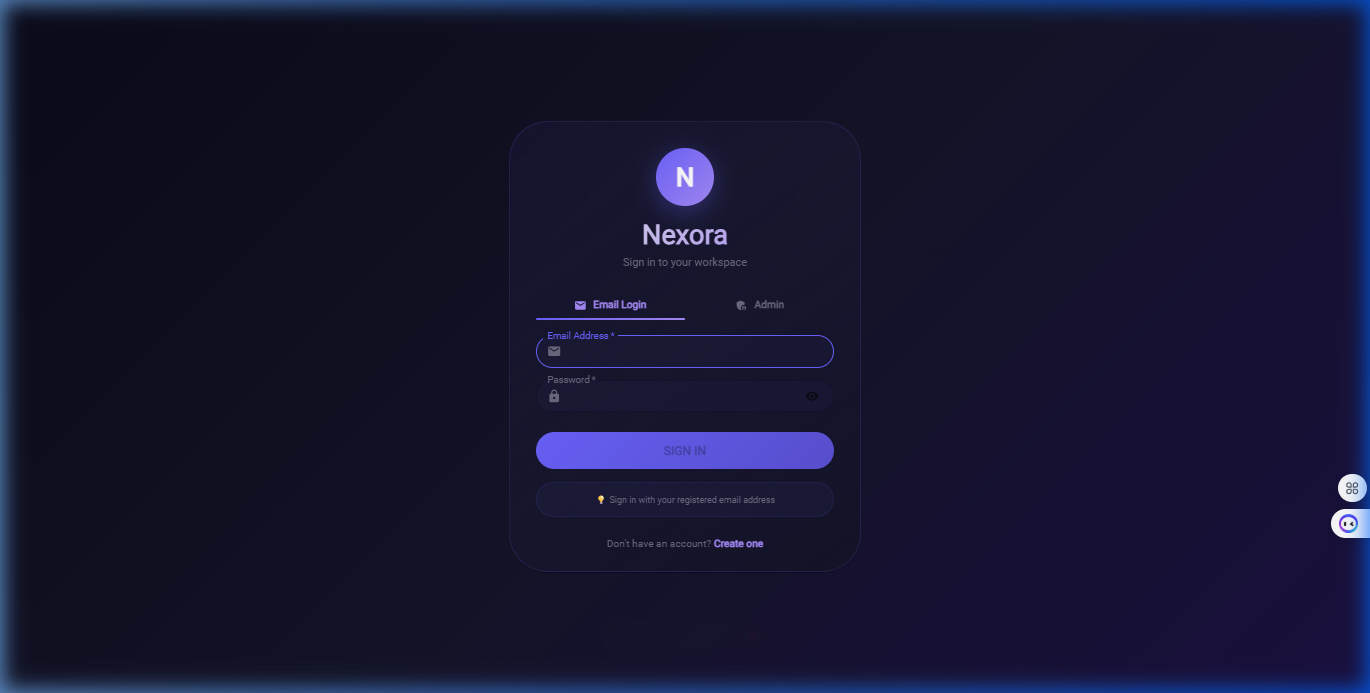
\includegraphics[width=0.95\textwidth]{screenshots/screenshot_login.png}
\caption{Exemple d'authentification : interface de connexion et flux sécurisé}
\label{fig:screenshot_login_alt}
\end{figure}

La Figure \ref{fig:screenshot_login_alt} fournit un second exemple d'écran d'authentification, utile pour documenter la cohérence UX et le rôle des variables d'environnement liées à la sécurité (clé JWT, durée d'expiration, etc.).

Cette interface illustre plusieurs aspects clés du système d'authentification :
\begin{itemize}
  \item \textbf{Champs de saisie sécurisés} : les champs email et mot de passe sont masqués pour éviter l'affichage en clair des informations sensibles
  \item \textbf{Validation côté client} : les formulaires vérifient le format des entrées avant soumission pour réduire les requêtes invalides
  \item \textbf{Feedback utilisateur} : les messages d'erreur sont affichés clairement en cas d'échec d'authentification
  \item \textbf{Intégration JWT} : après une connexion réussie, le token est stocké et utilisé pour les requêtes ultérieures
\end{itemize}

% =========================================================
% CHAPITRE 2 — ÉTAT DE L'ART
% =========================================================
\chapter{État de l'Art}

\section{Introduction}
Le marché de la gestion des compétences (Skills Management) et de la Talent Intelligence s'est fortement développé, sous l'effet de la transformation numérique et des exigences de mobilité interne. Les organisations cherchent à :
\begin{itemize}
  \item Réduire les délais de staffing
  \item Améliorer l'alignement compétences--projets
  \item Structurer des parcours de formation pilotés par des données
\end{itemize}

Néanmoins, l'efficacité d'une solution dépend de sa capacité à relier des informations hétérogènes :
\begin{itemize}
  \item Profils et compétences des employés
  \item Projets et contributions documentaires
  \item Interactions et formations
\end{itemize}

Une approche purement déclarative tend à produire un référentiel statique peu exploitable pour la recommandation et la découverte d'expertise. Il devient alors pertinent d'adopter des modèles capables de représenter des relations riches et évolutives.

Dans ce cadre, les bases de données orientées graphe et les approches hybrides (graph analytics + ML + IA générative) constituent un axe majeur : elles permettent de passer d'une description descriptive à une intelligence calculable et visualisable. La section suivante présente les fondements des bases orientées graphe.

\section{Les Bases de Données Orientées Graphe}
Une base orientée graphe modélise l'information sous forme de nœuds et de relations, chacun pouvant porter des propriétés. Cette représentation est particulièrement adaptée lorsque la relation est centrale :
\begin{itemize}
  \item Collaboration entre experts
  \item Co-occurrence de compétences
  \item Dépendances entre projets
  \item Liens entre documents
\end{itemize}

Les requêtes portent sur des motifs relationnels, des chemins et des voisinages.

À l'inverse, une base relationnelle excelle pour des transactions structurées, mais peut devenir coûteuse pour des analyses relationnelles profondes (multi-jointures). Les opérations suivantes sont moins naturelles en SQL et complexifient la maintenance :
\begin{itemize}
  \item Recherche de chemins
  \item Détection de communautés
  \item Traversées successives
\end{itemize}

Neo4j est pertinent pour NEXORA en raison de :
\begin{itemize}
  \item \textbf{Index-free adjacency} : navigation directe entre nœuds reliés
  \item \textbf{Cypher} : langage déclaratif pour les requêtes graphe
  \item \textbf{Extension APOC} : procédures et fonctions étendues
\end{itemize}

D'autres solutions existent (Neptune, ArangoDB, TigerGraph), mais Neo4j offre un compromis adapté entre maturité, expressivité et facilité d'intégration. Le tableau suivant synthétise la comparaison.

Cette comparaison met en évidence les avantages spécifiques d'une base de données orientée graphe pour NEXORA :
\begin{itemize}
  \item \textbf{Performance des traversées} : Neo4j utilise l'index-free adjacency pour naviguer directement entre nœuds reliés, sans jointures coûteuses
  \item \textbf{Expressivité des requêtes} : le langage Cypher permet d'exprimer des motifs relationnels complexes de manière naturelle
  \item \textbf{Flexibilité du schéma} : le modèle graphe s'adapte facilement à l'évolution des besoins sans migrations de schéma lourdes
  \item \textbf{Analytics intégrés} : les algorithmes de centralité et de détection de communautés sont natifs
\end{itemize}

\begin{table}[H]
\centering
\caption{Comparaison : Base Relationnelle vs Base Graphe}
\label{tab:rel_vs_graph}
\begin{tabular}{p{5cm} p{5cm} p{5cm}}
\toprule
\textbf{Critère} & \textbf{Relationnelle (SQL)} & \textbf{Graphe (Neo4j)} \\
\midrule
Modèle & Tables, lignes, jointures & Nœuds, relations, propriétés \\
Exploration relationnelle & Coûteux (multi-JOIN) & Natif (traversées) \\
Chemins / motifs & Non naturel & Expressif (Cypher) \\
Analytics & Externe & Centralité, motifs, voisinage \\
Cas d'usage & Transactions, reporting & Recommandation, connaissance \\
\bottomrule
\end{tabular}
\end{table}

\section{Frameworks Web Modernes}
Le choix des frameworks web conditionne la performance, la maintenabilité et la qualité du contrat d'API. FastAPI, retenu dans NEXORA, se distingue par la génération OpenAPI automatique, le typage et la validation (Pydantic), ainsi que la compatibilité ASGI, utile pour les endpoints asynchrones et les WebSocket.

Django constitue un framework robuste, mais plus orienté monolithe et rendu serveur, ce qui peut alourdir une démarche API-First. Express (Node.js) est flexible, mais impose une discipline supplémentaire pour atteindre un niveau équivalent de validation et de documentation. Dans NEXORA, la cohérence du contrat et l'intégration des modules ML (Python) ont motivé l'option FastAPI.

Les avantages spécifiques de FastAPI pour ce projet incluent :
\begin{itemize}
  \item \textbf{Documentation automatique} : OpenAPI/Swagger généré automatiquement pour tous les endpoints
  \item \textbf{Validation stricte} : Pydantic valide les entrées/sorties avec des types Python natifs
  \item \textbf{Performance} : support ASGI pour les opérations asynchrones et WebSocket
  \item \textbf{Intégration ML} : écosystème Python riche (scikit-learn, pandas, numpy)
\end{itemize}

Côté frontend, React 18 et TypeScript offrent une base solide pour une SPA riche. L'écosystème MUI apporte des composants réutilisables et une cohérence UI, tandis que Vite optimise le build. La visualisation 3D, rendue via WebGL, renforce la capacité d'exploration de la connaissance organisationnelle.

Les choix technologiques pour le frontend reposent sur plusieurs critères :
\begin{itemize}
  \item \textbf{Performance} : React 18 avec automatic batching réduit les re-rendus inutiles
  \item \textbf{Type safety} : TypeScript détecte les erreurs dès la compilation
  \item \textbf{Cohérence UI} : Material-UI fournit des composants prêts à l'emploi et thématiques
  \item \textbf{Vitesse de développement} : Vite accélère le build et le hot reload
  \item \textbf{Visualisation avancée} : WebGL permet le rendu 3D performant dans le navigateur
\end{itemize}

\section{Solutions de Gestion des Connaissances Existantes}
Les solutions concurrentes proposent des fonctionnalités de cartographie et de recommandation, mais diffèrent sur la transparence des modèles et l'ouverture :
\begin{itemize}
  \item \textbf{365Talents} : capacités IA avancées, mais graphe non explicitable
  \item \textbf{Workday Skills Cloud} : ontologie massive et intégration SI forte, mais écosystème propriétaire
  \item \textbf{Cornerstone OnDemand} : riche en LMS, mais moins orienté cartographie relationnelle
  \item \textbf{LinkedIn Talent Insights} : puissance analytique sur données externes, pas de cartographie interne
  \item \textbf{Skills Base} : accessible mais largement déclaratif, peu orienté IA
\end{itemize}

Ces constats motivent le positionnement de NEXORA, dont la valeur ajoutée repose sur :
\begin{itemize}
  \item \textbf{Graphe natif explicite} : relations modélisées et navigables pour l'explicabilité
  \item \textbf{Visualisation 3D immersive} : exploration interactive du graphe organisationnel
  \item \textbf{Chaîne IA hybride} : combinaison d'algorithmes classiques et de LLM
  \item \textbf{Architecture ouverte} : API-First et technologies open source
  \item \textbf{Mode dégradé} : fallback JSONL pour continuité de service
\end{itemize}

\section{Positionnement de NEXORA}
NEXORA combine :
\begin{itemize}
  \item Un graphe Neo4j pour la modélisation des relations
  \item Une visualisation 3D WebGL pour l'exploration interactive
  \item Une chaîne IA hybride (PageRank, TF-IDF + cosinus, filtrage collaboratif, classification, assistant LLM)
\end{itemize}

Cette combinaison fournit plusieurs modes d'accès à la connaissance :
\begin{itemize}
  \item Exploration visuelle du graphe
  \item Recherche sémantique d'experts et documents
  \item Recommandation personnalisée
  \item Conversation avec l'assistant Veda
\end{itemize}

Les différenciateurs clés de NEXORA sont :
\begin{itemize}
  \item \textbf{Centralité du graphe} : relations explicitement modélisées pour calcul de chemins, détection de ponts inter-départements et explicabilité
  \item \textbf{Hybridation ML + LLM} : résultats produits par scores quantitatifs (cosinus, PageRank) et contextualisés via Veda
  \item \textbf{Intégration Big Data} : PySpark + streaming simulé, rarement mis en œuvre dans des projets académiques
\end{itemize}

Il convient toutefois de noter des limites :
\begin{itemize}
  \item Le streaming est simulé (pas de cluster Kafka réel)
  \item Le fallback JSONL doit être gouverné pour éviter des divergences
\end{itemize}

Ces aspects sont traités comme des défis d'ingénierie dans la suite du rapport.

% =========================================================
% CHAPITRE 3 — ARCHITECTURE DU SYSTÈME
% =========================================================
\chapter{Architecture du Système}

\section{Vue d'Ensemble}
NEXORA adopte une architecture 3-tiers :
\begin{itemize}
  \item \textbf{Couche présentation} : React avec TypeScript pour l'interface utilisateur
  \item \textbf{Couche métier} : FastAPI avec Python pour la logique métier et l'API
  \item \textbf{Couche données} : Neo4j (graphe), JSONL (fallback), résultats Spark (batch)
\end{itemize}

Cette séparation vise à :
\begin{itemize}
  \item Limiter le couplage entre composants
  \item Faciliter l'évolution indépendante des couches
  \item Permettre la montée en charge horizontale
\end{itemize}

Le backend est conçu pour rester majoritairement stateless, ce qui favorise la scalabilité.

Dans cette organisation, chaque couche a une responsabilité claire :
\begin{itemize}
  \item \textbf{Couche présentation} : expérience utilisateur (navigation, visualisation, interaction)
  \item \textbf{Couche métier} : point d'entrée unique aux données et traitements (recherche, recommandation, collaboration)
  \item \textbf{Couche données} : concilier analyse relationnelle (Neo4j) et reproductibilité (JSONL + outputs Spark)
\end{itemize}

Cette séparation facilite aussi le travail en binôme : les développements frontend peuvent progresser sur des contrats d'API stables pendant que la modélisation graphe et les modules IA/Big Data évoluent côté backend.

\Needspace{18\baselineskip}
\begin{figure}[H]
\centering
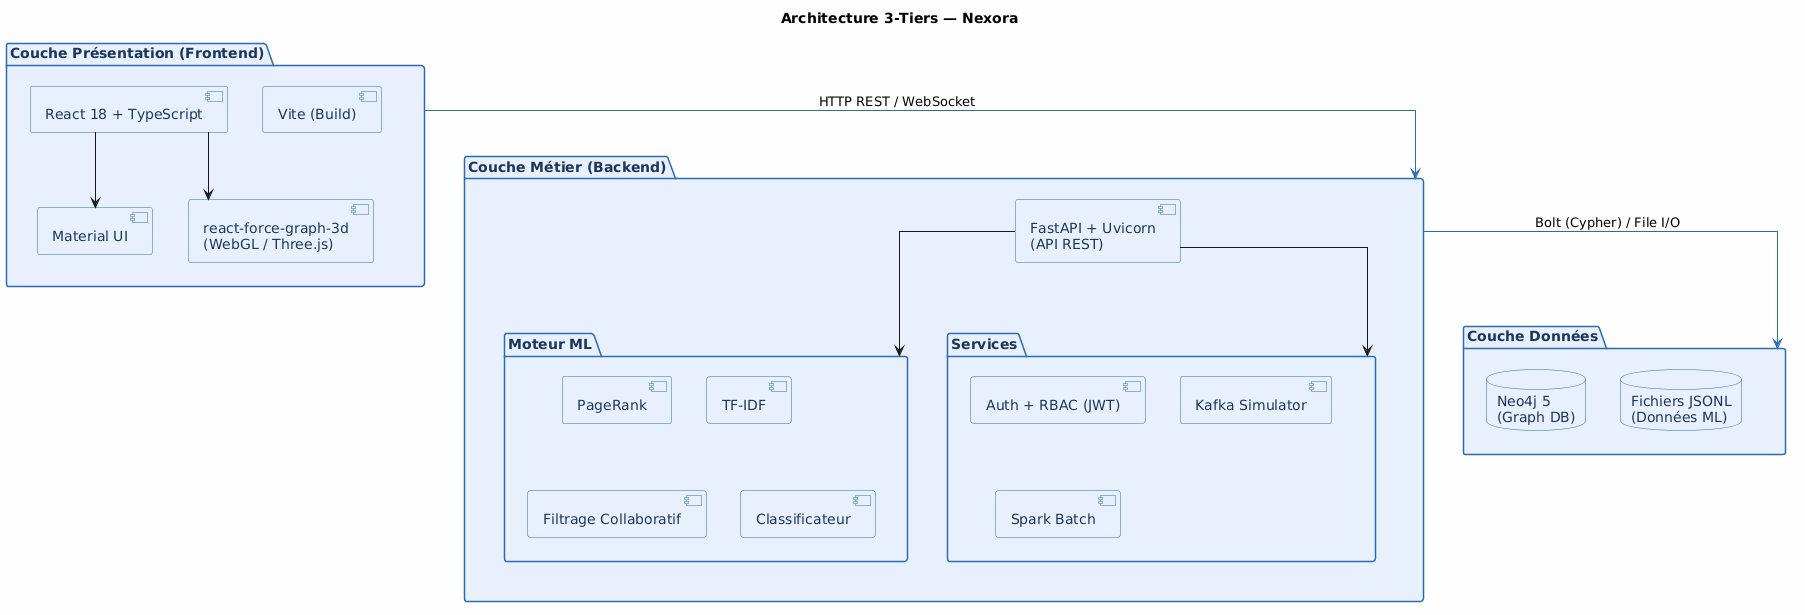
\includegraphics[width=0.95\textwidth]{screenshots/08_architecture_3tiers.png}
\caption{Architecture 3-tiers de NEXORA}
\label{fig:arch_3tiers}
\end{figure}

La Figure \ref{fig:arch_3tiers} synthétise l'organisation du système en trois couches. Le frontend (React) consomme des endpoints REST et WebSocket exposés par le backend (FastAPI), lequel orchestre l'accès aux données Neo4j, aux fichiers JSONL de repli et aux résultats Big Data (outputs Spark).

Cette architecture en couches présente plusieurs avantages structurants :
\begin{itemize}
  \item \textbf{Backend comme façade} : centralise l'authentification (JWT), applique les règles d'accès (RBAC) et expose une API homogène aux modules (graphe, IA, Big Data, collaboration)
  \item \textbf{Couche données hybride} : Neo4j apporte les traversées et requêtes relationnelles, tandis que les JSONL garantissent un mode dégradé pour la démonstration et la reproductibilité
  \item \textbf{Séparation en services} : facilite la conteneurisation (Docker Compose), chaque composant évolue et se déploie indépendamment via des contrats d'API stables
  \item \textbf{Scalabilité} : backend stateless pour montée en charge horizontale, cache pour requêtes fréquentes, WebSocket pour éviter le polling
\end{itemize}

Le principe API-First structure l'intégration :
\begin{itemize}
  \item Routes exposées sous \texttt{/api/}
  \item Documentation automatique via OpenAPI
  \item Communications temps réel (messagerie, workspaces) via WebSocket pour interactions bidirectionnelles
\end{itemize}

Cette approche facilite l'intégration avec des systèmes tiers :
\begin{itemize}
  \item Système RH peut interroger l'API pour des statistiques sur les compétences
  \item Outil de gestion de projet peut récupérer des informations sur les experts disponibles
  \item Documentation OpenAPI comme contrat d'interface pour les développeurs externes
\end{itemize}

L'adoption de standards web (REST, WebSocket, JSON) garantit :
\begin{itemize}
  \item Compatibilité maximale avec les navigateurs modernes et frameworks JavaScript
  \item Frontend React peut consommer les API via Axios ou Fetch
  \item Communication WebSocket gérée par bibliothèques spécialisées avec reconnexion automatique
  \item Standardisation réduit la courbe d'apprentissage et facilite l'onboarding technique
\end{itemize}

Le déploiement via Docker Compose rend l'environnement reproductible :
\begin{itemize}
  \item Frontend servi via Nginx
  \item Neo4j isolé en service dédié
  \item Healthcheck vérifie Neo4j avant le démarrage du backend
\end{itemize}

Cette approche conteneurisée présente des avantages opérationnels :
\begin{itemize}
  \item \textbf{Élimination des problèmes de configuration} : encapsulation des dépendances dans les images Docker, évite le "ça marche sur ma machine"
  \item \textbf{Isolation stricte} : chaque service dans son propre conteneur avec ses variables d'environnement, évite les conflits de versions
  \item \textbf{Orchestration simplifiée} : Docker Compose définit les dépendances, réseaux, volumes et politiques de redémarrage
\end{itemize}

Les healthchecks intégrés assurent :
\begin{itemize}
  \item Services ne démarrent que lorsque leurs dépendances sont prêtes
  \item Backend attend que Neo4j réponde correctement avant initialisation
  \item Frontend Nginx attend que le backend soit opérationnel avant de servir l'application
  \item Évite les erreurs 502/503 lors de l'accès initial
  \item Robustesse opérationnelle pour démonstrations et présentations
\end{itemize}

\section{Structure du Projet}
Le backend est organisé par routeurs (\texttt{backend/app/routers}) couvrant les domaines fonctionnels :
\begin{itemize}
  \item Experts, documents, graphe, learning, dashboard, auth
  \item IA, Big Data, feed, network, messaging, jobs
  \item Notifications, gamification, skillmap, workspaces, simulateur Kafka
\end{itemize}

Les modules ML sont isolés sous \texttt{backend/app/ml} et les jobs Spark sous \texttt{backend/spark}.

Le frontend (\texttt{frontend/src}) est organisé en :
\begin{itemize}
  \item Pages dédiées aux modules : Feed, GraphVisualization, LearningPath, Messaging, TeamBuilder, TeamWorkspace
  \item Pages d'authentification
  \item Composants réutilisables
  \item Routage centralisé dans \texttt{App.tsx}
\end{itemize}

Les données sont fournies au format JSONL dans \texttt{data/} :
\begin{itemize}
  \item Employees, skills, projects, documents
  \item Catalogues additionnels : companies, technologies
\end{itemize}

Cette structuration vise à limiter la complexité :
\begin{itemize}
  \item Chaque sous-système possède ses fichiers, routes et modèles clairement définis
  \item Backend : découpage en routeurs réduit les conflits, améliore la lisibilité (un domaine fonctionnel = un point de maintenance)
  \item Frontend : séparation pages/composants évite la duplication, factorise l'UI (layout, navigation, formulaires, tableaux)
  \item Facilite l'ajout de fonctionnalités sans remettre en cause l'architecture existante
\end{itemize}

Au niveau du backend :
\begin{itemize}
  \item Chaque router est un module autonome avec ses propres modèles Pydantic, services métier et dépendances
  \item Modularité permet de tester chaque router indépendamment
  \item Facilite la collaboration entre développeurs (travail parallèle sur différents routeurs)
  \item Modèles partagés extraits dans des modules communs pour éviter la duplication
\end{itemize}

Concernant le frontend :
\begin{itemize}
  \item Composants de base (boutons, formulaires, tableaux, cartes) définis dans \texttt{components}
  \item Réutilisabilité garantit uniformité visuelle et réduit le code dupliqué
  \item Pages encapsulent la logique spécifique tout en s'appuyant sur des composants génériques
  \item Lazy loading : seuls les composants nécessaires sont chargés lors de la navigation
\end{itemize}

\section{Communication entre Couches}
Le frontend communique avec le backend via HTTP REST, avec transport de JWT dans l'en-tête \texttt{Authorization}. Les pages consomment les endpoints pour alimenter les recherches, dashboards et la visualisation 3D. L'authentification est validée côté backend, puis les dépendances RBAC filtrent l'accès.

Les fonctionnalités temps réel s'appuient sur WebSocket : messagerie (endpoint par utilisateur) et workspaces (endpoint par workspace et utilisateur). Ce canal supporte des signaux d'interface (typing indicator) et améliore l'expérience.

Le backend communique avec Neo4j via Bolt et exécute des requêtes Cypher. Lorsque Neo4j n'est pas disponible, certaines routes utilisent un mécanisme de fallback basé sur les données JSONL.

Le protocole Bolt, utilisé pour la communication entre le backend et Neo4j, est optimisé pour les performances :
\begin{itemize}
  \item Pipelining des requêtes pour réduire la latence
  \item Compression des données pour minimiser le transfert réseau
  \item Pool de connexions automatique géré par le driver Neo4j Python
  \item Réutilisation des connexions existantes
\end{itemize}

Les requêtes Cypher sont :
\begin{itemize}
  \item Paramétrées pour éviter les injections SQL
  \item Optimisées grâce à l'utilisation d'index sur les propriétés fréquemment recherchées (email, nom, compétences)
\end{itemize}

Le mécanisme de fallback JSONL est conçu pour être transparent pour l'utilisateur :
\begin{itemize}
  \item Lorsqu'une requête Neo4j échoue, le backend tente automatiquement de répondre en utilisant les fichiers JSONL stockés localement
  \item Particulièrement utile pour les démonstrations en environnement contraint (connexion internet limitée, base de données non disponible)
  \item Permet de valider la logique métier indépendamment de l'infrastructure de base de données
  \item Note : ce mode dégradé ne supporte pas toutes les fonctionnalités (notamment les traversées de graphe complexes et les calculs de centralité en temps réel)
\end{itemize}

Pour préserver un comportement homogène :
\begin{itemize}
  \item Réponses API normalisées (codes HTTP, schémas Pydantic)
  \item Documentation OpenAPI comme référence unique pour l'intégration
  \item Appels sensibles protégés par des dépendances d'autorisation
  \item Échanges temps réel gérés par un Connection Manager
  \item Conception limite les effets de bord : erreur Neo4j ou timeout externe produit une réponse contrôlée plutôt qu'un échec global
\end{itemize}

La normalisation des réponses API garantit :
\begin{itemize}
  \item Frontend peut traiter les réponses de manière prévisible
  \item Codes HTTP utilisés de manière sémantique :
    \begin{itemize}
      \item 200 pour les succès
      \item 201 pour les créations
      \item 400 pour les erreurs de validation
      \item 401 pour l'authentification manquante
      \item 403 pour l'autorisation refusée
      \item 404 pour les ressources introuvables
      \item 500 pour les erreurs serveur inattendues
    \end{itemize}
  \item Schémas Pydantic définissent la structure des données en entrée et en sortie
  \item Validation automatique et génération de documentation
  \item Réduction des erreurs d'intégration et facilitation du débogage
\end{itemize}

Le Connection Manager pour WebSocket joue un rôle crucial :
\begin{itemize}
  \item Maintient une registry des connexions actives
  \item Associe chaque connexion à un utilisateur et/ou un workspace
  \item Gère les événements de connexion et de déconnexion
  \item Détecte la déconnexion et nettoie les ressources associées (évite les fuites de mémoire)
  \item Gère la diffusion des messages : identifie tous les utilisateurs connectés à un workspace et leur envoie le message
\end{itemize}

\section{Patterns de Conception Utilisés}
Les patterns de conception utilisés dans NEXORA sont :
\begin{itemize}
  \item \textbf{Singleton} : pour le driver Neo4j et les caches de modèles ML
  \item \textbf{Dependency Injection} : via \texttt{Depends} (FastAPI) pour composer l'authentification et l'autorisation
  \item \textbf{Connection Manager} : pour les composants WebSocket
  \item \textbf{Strategy} : pour les modules ML (recommandation, classification, embeddings, PageRank, GraphRAG)
  \item \textbf{Factory} : pour la génération de données paramétrable (small/medium/large)
\end{itemize}

Ces patterns contribuent à la testabilité et à la maintenabilité :
\begin{itemize}
  \item Dépendances (auth, base de données, paramètres) peuvent être substituées ou simulées lors des tests
  \item Stratégies ML peuvent évoluer indépendamment du reste de l'API
  \item Ajout d'un nouvel algorithme (ou variante) sans modifier les routes consommatrices
  \item Remplacement d'une implémentation derrière une interface ou un service, avec conservation des mêmes contrats d'entrée/sortie
\end{itemize}

Le pattern Singleton :
\begin{itemize}
  \item Appliqué au driver Neo4j et aux caches de modèles ML
  \item Garantit qu'il n'existe qu'une seule instance de ces ressources critiques
  \item Évite la surcharge mémoire liée à la création de connexions multiples
  \item Assure la cohérence des données (cache de modèles ML reste synchronisé)
  \item Driver Neo4j Singleton gère automatiquement le pool de connexions
  \item Améliore significativement les performances des requêtes Cypher
\end{itemize}

La Dependency Injection via \texttt{Depends} :
\begin{itemize}
  \item Élément central de l'architecture FastAPI
  \item Chaque endpoint déclare ses dépendances (authentification, base de données, services métier)
  \item FastAPI résout automatiquement les dépendances avant l'exécution
  \item Permet de décorer les endpoints avec des gardes d'autorisation sans modifier la logique métier
  \item Facilite les tests : dépendances remplacées par des mocks ou des stubs
\end{itemize}

Le pattern Strategy :
\begin{itemize}
  \item Visible dans les modules ML
  \item Chaque algorithme de recommandation, classification ou calcul de centralité est une stratégie interchangeable
  \item Système de recommandation peut utiliser différentes approches (filtrage collaboratif, PageRank personnalisé, similarité cosinus)
  \item Consommateur (endpoint API) n'a pas à connaître les détails de l'implémentation
  \item Flexibilité pour expérimenter rapidement de nouveaux algorithmes
  \item Comparaison des performances sans impacter l'interface utilisateur
\end{itemize}

\section{Flux de Données Complet}
Le flux global de données comprend :
\begin{itemize}
  \item \textbf{Génération} : fichiers JSONL via un script paramétrable (seed fixe)
  \item \textbf{Ingestion} : dans Neo4j via des scripts Cypher
  \item \textbf{Traitement ML} : modules ML produisent des recommandations et analyses
  \item \textbf{Batch Spark} : jobs Spark calculent des agrégations batch
  \item \textbf{Consommation} : résultats stockés dans \texttt{backend/spark/output} et consommés par les endpoints Big Data
\end{itemize}

Ce flux est conçu pour être \textbf{traçable} :
\begin{itemize}
  \item Relancer la génération avec le même seed pour reproduire les données
  \item Vérifier que l'ingestion et les traitements produisent des résultats cohérents
  \item Important pour un projet académique
  \item Utile en contexte industriel (rejeu d'un pipeline, vérification post-correction, validation de performances)
  \item Facilite la mise au point de la visualisation 3D et des modules de recommandation
\end{itemize}

La génération de données JSONL :
\begin{itemize}
  \item Utilise un algorithme pseudo-aléatoire avec une seed fixe
  \item Garantit que chaque exécution produit exactement le même jeu de données
  \item Contraintes de cohérence :
    \begin{itemize}
      \item Employé associé à des compétences pertinentes pour son département
      \item Projet implique des employés avec les compétences requises
      \item Documents liés aux projets correspondants
    \end{itemize}
  \item Cohérence sémantique essentielle pour des résultats pertinents et une visualisation interprétable
\end{itemize}

L'ingestion dans Neo4j :
\begin{itemize}
  \item Via des scripts Cypher qui créent les nœuds (Employee, Skill, Project, Document, Company, Technology)
  \item Créent les relations (HAS\_SKILL, WORKS\_ON, CONTRIBUTED\_TO, etc.)
  \item Scripts idempotents : peuvent être réexécutés sans créer de doublons
  \item Facilite les mises à jour incrémentales
  \item Contraintes d'unicité définies pour garantir l'intégrité des données (ex: un employé ne peut avoir qu'un seul email)
\end{itemize}

Les modules ML exploitent ces données pour :
\begin{itemize}
  \item Calculer des métriques et des recommandations
  \item PageRank : traverse le graphe pour identifier les experts les plus centraux
  \item Similarité TF-IDF : analyse les descriptions de compétences pour trouver des profils similaires
  \item Calculs effectués à la demande (mode interactif) ou en batch via Spark
\end{itemize}

Les jobs Spark traitent les données JSONL pour :
\begin{itemize}
  \item Produire des agrégations batch :
    \begin{itemize}
      \item Statistiques sur la distribution des compétences
      \item Scores de popularité des documents
      \item Classements des experts par département
    \end{itemize}
  \item Résultats stockés dans des fichiers JSON dans \texttt{backend/spark/output}
  \item Consommés par les endpoints Big Data
  \item Approche batch permet de traiter de gros volumes efficacement
  \item Réduit la charge sur Neo4j lors des requêtes fréquentes
\end{itemize}

\begin{figure}[H]
\centering
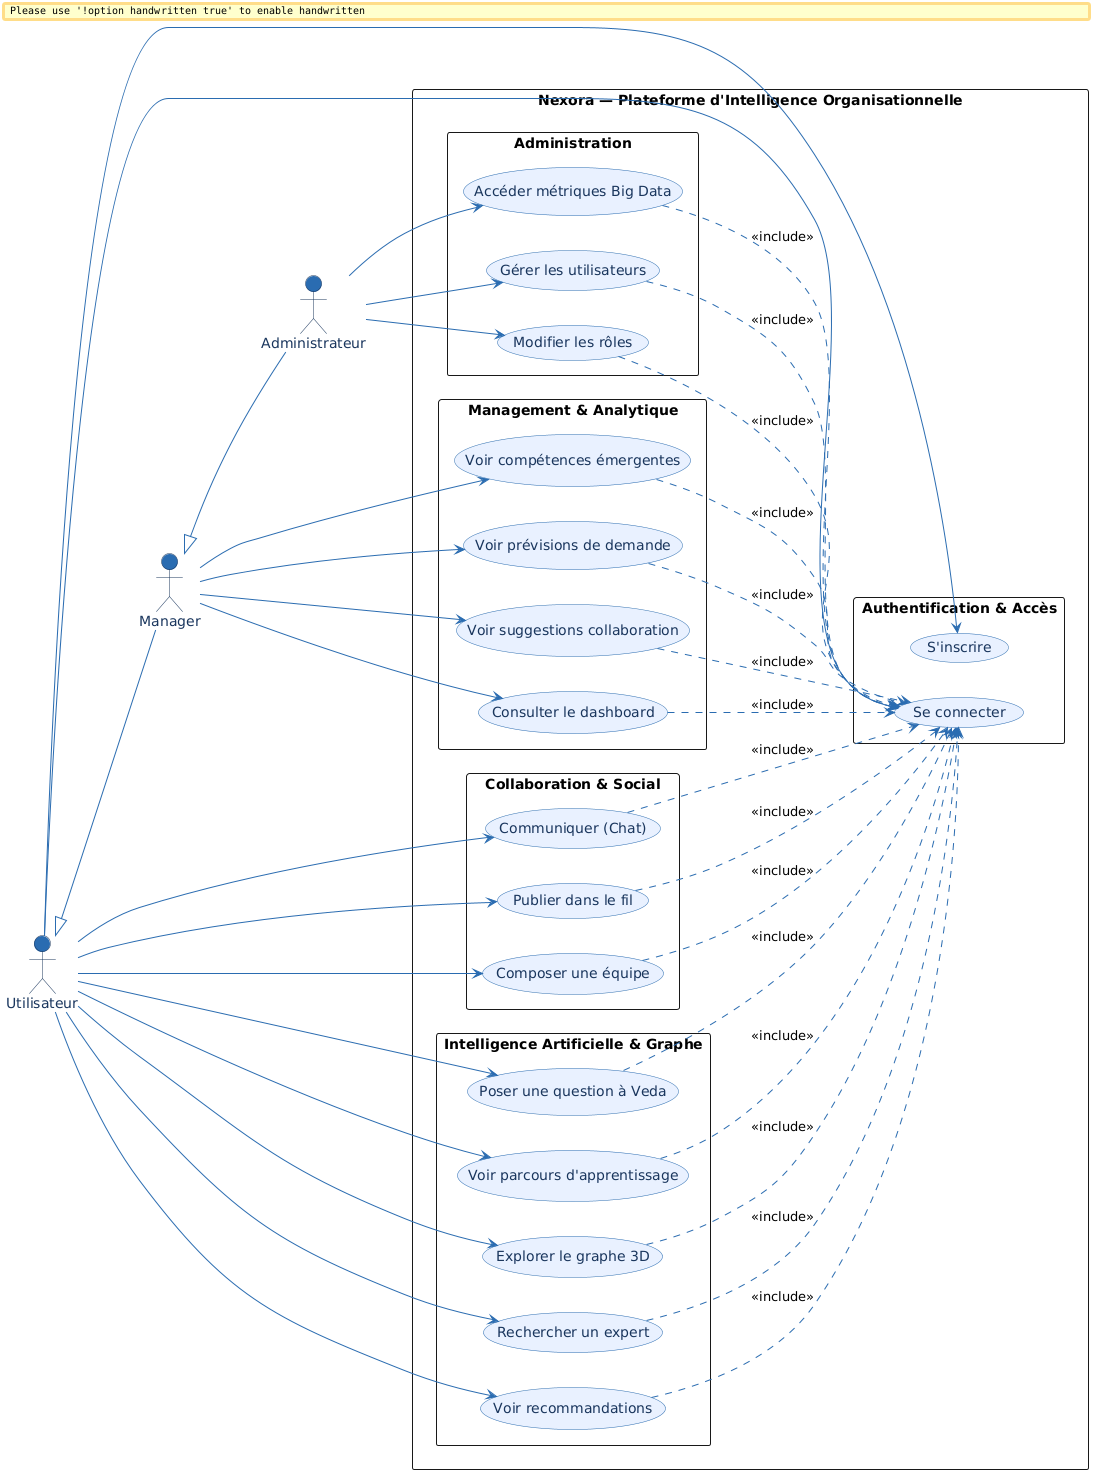
\includegraphics[width=0.95\textwidth]{screenshots/01_use_case.png}
\caption{Cas d'usage principaux de NEXORA}
\label{fig:use_case}
\end{figure}

La Figure \ref{fig:use_case} regroupe les interactions principales : authentification, recherche d'experts et de documents, recommandations, exploration du graphe 3D, ainsi que l'assistant conversationnel. Ces cas d'usage guident la priorisation des endpoints et la conception de l'interface.

Les cas d'usage principaux de NEXORA sont :
\begin{itemize}
  \item \textbf{Authentification} : inscription, connexion, gestion des sessions JWT
  \item \textbf{Recherche d'experts} : recherche sémantique, filtrage par compétences, classement PageRank
  \item \textbf{Recherche de documents} : recherche textuelle, classification par thématique, recommandations
  \item \textbf{Recommandations} : suggestions de compétences, d'experts, de formations
  \item \textbf{Exploration 3D} : navigation interactive dans le graphe organisationnel
  \item \textbf{Assistant conversationnel} : chatbot Veda pour interrogation en langage naturel
  \item \textbf{Collaboration} : messagerie temps réel, workspaces d'équipe, constitution d'équipes
\end{itemize}

\begin{figure}[H]
\centering
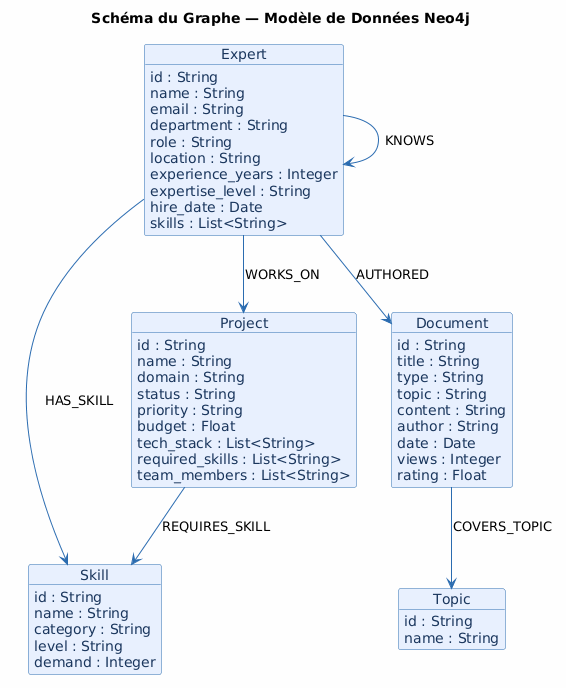
\includegraphics[width=0.95\textwidth]{screenshots/07_graph_schema.png}
\caption{Schéma et relations clés du graphe (représentation)}
\label{fig:graph_schema}
\end{figure}

La Figure \ref{fig:graph_schema} illustre les entités structurantes (experts, compétences, projets, documents) et les relations qui permettent l'explicabilité (parcours de graphe) et les calculs de ranking. Ce modèle alimente les requêtes Cypher, la visualisation 3D et les algorithmes de recommandation.

Les entités principales du graphe sont :
\begin{itemize}
  \item \textbf{Expert (Employee)} : employé avec compétences, département, rôle, localisation
  \item \textbf{Skill} : compétence avec catégorie, niveau de demande, description
  \item \textbf{Project} : projet avec statut, date, stack technologique, compétences requises
  \item \textbf{Document} : document avec type, topic, rating, vues, auteur
  \item \textbf{Company} : entreprise avec secteur, localisation, taille
  \item \textbf{Technology} : technologie avec catégorie, popularité
\end{itemize}

Les relations clés incluent :
\begin{itemize}
  \item HAS\_SKILL : expert possède une compétence (avec niveau)
  \item WORKS\_ON : expert participe à un projet
  \item CONTRIBUTED\_TO : expert a contribué à un document
  \item REQUIRES\_SKILL : projet nécessite une compétence
  \item RELATED\_TO : document lié à un projet ou une compétence
\end{itemize}

\begin{figure}[H]
\centering
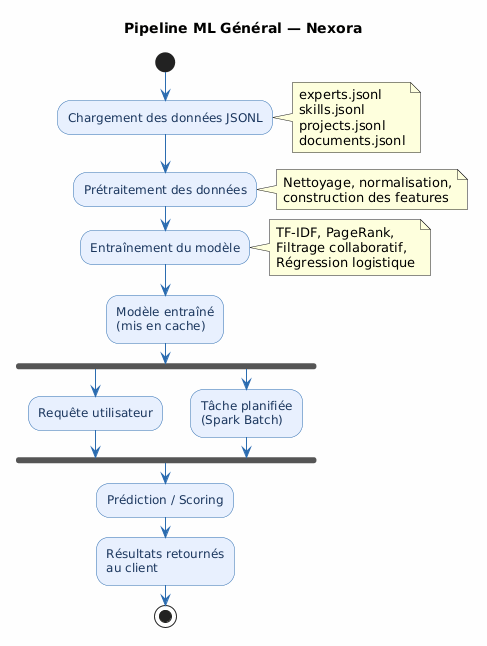
\includegraphics[width=0.95\textwidth]{screenshots/09_pipeline_ml.png}
\caption{Pipeline d'analyse et modules IA (vue d'ensemble)}
\label{fig:pipeline_ml}
\end{figure}

La Figure \ref{fig:pipeline_ml} résume la chaîne de traitement : ingestion/normalisation, représentation textuelle (TF-IDF), classification et scoring, puis exposition via l'API. Elle met en évidence le rôle des sorties batch (Spark) et des mécanismes de repli lorsque des composants externes sont indisponibles.

Le pipeline ML de NEXORA comprend les étapes suivantes :
\begin{itemize}
  \item \textbf{Ingestion} : chargement des données JSONL et création des nœuds/relations Neo4j
  \item \textbf{Normalisation} : nettoyage des textes, tokenisation, lemmatisation
  \item \textbf{Représentation} : calcul des vecteurs TF-IDF pour les textes
  \item \textbf{Classification} : catégorisation automatique des documents par thématique
  \item \textbf{Scoring} : calcul des scores de similarité et de centralité (PageRank)
  \item \textbf{Exposition} : exposition des résultats via l'API REST
\end{itemize}

Les mécanismes de fallback et de robustesse incluent :
\begin{itemize}
  \item Fallback JSONL si Neo4j indisponible
  \item Cache en mémoire pour les calculs fréquents
  \item Fallback rule-based si LLM (Groq) indisponible
  \item Batch Spark pour les agrégations lourdes
\end{itemize}

Le simulateur Kafka illustre un mode streaming par production d'événements. L'ensemble des résultats est exposé via l'API et rendu dans le frontend : dashboards, recherche, visualisation 3D, chat Veda, et modules collaboratifs.

\section{Gestion des Erreurs}
La gestion des erreurs repose sur des exceptions FastAPI traduites en codes HTTP adaptés (401, 403, 404, 422, 500). Les validations Pydantic renforcent la robustesse des entrées. En sécurité, un mécanisme de rate limiting est appliqué au login.

Un mécanisme de fallback JSONL est présent lorsque Neo4j est indisponible, améliorant la continuité de démonstration. Cependant, il impose une gouvernance stricte pour éviter des divergences.

L'objectif principal est de garantir une \textbf{dégradation contrôlée}. Lorsque la dépendance critique (base graphe ou service externe) n'est pas accessible, l'API privilégie une réponse partielle ou alternative plutôt qu'une rupture. Cette approche améliore l'expérience utilisateur (les pages restent fonctionnelles) et facilite la démonstration : on peut montrer la logique métier même en cas d'indisponibilité temporaire d'un composant.

% =========================================================
% CHAPITRE 4 — GESTION DE PROJET
% =========================================================
\addtocontents{toc}{\protect\Needspace{6\baselineskip}}
\clearpage
\chapter{Gestion de Projet}

\section{Objectifs et Périmètre}
Cette section présente la démarche de \textbf{gestion de projet} appliquée à NEXORA. L'objectif est de montrer comment le travail a été cadré, découpé, planifié et piloté afin de produire un livrable complet (backend, frontend, base graphe, IA/Big Data, déploiement et documentation). Le périmètre couvre :

\begin{itemize}
  \item la définition des objectifs et des contraintes (sécurité, performance, robustesse),
  \item le découpage en lots et la planification par dépendances,
  \item la répartition des responsabilités au sein du binôme,
  \item l'anticipation des risques et la mise en place de mitigations.
\end{itemize}

\section{Charte de Projet (Cadrage)}
Le cadrage de NEXORA a consisté à formaliser le \textbf{besoin}, les \textbf{objectifs}, les \textbf{parties prenantes} et les \textbf{critères d'acceptation}. Le problème adressé est la fragmentation de la connaissance des compétences dans les organisations, ce qui complexifie l'identification d'experts, la collaboration et la capitalisation documentaire.

Les objectifs ont été définis autour d'un socle fonctionnel (recherche d'experts et documents, visualisation graphe), d'un socle d'intelligence (recommandations, classification, ranking), et d'un socle d'industrialisation (sécurité, déploiement reproductible, tests, documentation).

\section{Cahier des Charges (Expression des Besoins)}
Les besoins de NEXORA ont été exprimés selon une logique \textbf{fonctionnelle} et \textbf{non fonctionnelle}, afin d'assurer une cohérence entre le produit attendu et l'implémentation.

Le cahier des charges de NEXORA peut être synthétisé autour de :
\begin{itemize}
  \item \textbf{Fonctionnel} : recherche experts/documents, visualisation graphe, recommandations, collaboration (messaging/workspaces),
  \item \textbf{Non fonctionnel} : sécurité JWT+RBAC, robustesse (fallback), performance (cache ML, sous-graphes),
  \item \textbf{Livrables} : application conteneurisée, documentation API (Swagger), rapport et démonstration.
\end{itemize}

\section{Découpage (WBS) et Lots}
Pour NEXORA, le découpage en sous-problèmes a été déterminant pour maîtriser la complexité (graphe + IA + UI + DevOps). Le WBS a été construit pour obtenir des incréments démontrables, en limitant les intégrations tardives et en rendant explicites les dépendances entre modules.

Ce découpage favorise l'alignement entre architecture technique et gouvernance du projet : chaque lot produit un incrément démontrable et testable.

\begin{table}[H]
\centering
\caption{WBS (Work Breakdown Structure) spécifique à NEXORA}
\label{tab:wbs_nexora}
\begin{tabular}{p{2.8cm} p{5cm} p{6.5cm}}
\toprule
\textbf{Lot} & \textbf{Sous-lots} & \textbf{Livrables / critères de sortie} \\
\midrule
Lot 1 & Données \& Graphe & Génération JSONL (échelles), modélisation Neo4j, requêtes Cypher, endpoints graphe pour visualisation 3D \\
Lot 2 & Backend API & FastAPI (routeurs), sécurité JWT+RBAC, endpoints IA (TF-IDF, classification, PageRank), endpoints Big Data (Spark outputs + fallback), WebSocket (messaging/workspaces) \\
Lot 3 & Frontend & Pages React (routing), ProtectedRoute, TopNavBar, intégration API, visualisation 3D, chatbot Veda, écrans de recherche/recommandation \\
Lot 4 & Qualité \& Déploiement & Docker Compose, healthchecks, tests backend (Pytest), Swagger opérationnel, stabilité des erreurs (401/403/422/500), rapport final \\
\bottomrule
\end{tabular}
\end{table}

\section{Planification : Diagramme de Gantt et Chemin Critique}

\subsection{Diagramme de Gantt}
Le diagramme de Gantt ci-dessous illustre l'ordonnancement des principales tâches du projet NEXORA sur 8 semaines. Les barres rouges identifient le \textbf{chemin critique} (marge nulle) et les barres bleues les tâches disposant d'une marge. Les flèches matérialisent les dépendances.

\definecolor{critbar}{RGB}{220,60,60}
\definecolor{noncritbar}{RGB}{70,130,200}

\begin{figure}[H]
\centering

\resizebox{\textwidth}{!}{%
\begin{ganttchart}[
  hgrid,
  vgrid,
  x unit=0.75cm,
  y unit title=0.55cm,
  y unit chart=0.55cm,
  title/.style={fill=blue!15},
  title label font=\bfseries\scriptsize,
  bar label font=\scriptsize,
  group label font=\bfseries\scriptsize,
  milestone/.style={fill=red!60, shape=star},
  link/.style={->, thick, critbar},
  group/.style={fill=green!25}
]{1}{8}
\gantttitle{Calendrier du projet NEXORA (semaines)}{8} \\
\gantttitle{S1}{1} \gantttitle{S2}{1} \gantttitle{S3}{1} \gantttitle{S4}{1}
\gantttitle{S5}{1} \gantttitle{S6}{1} \gantttitle{S7}{1} \gantttitle{S8}{1} \\
% --- Lot 1 : Cadrage ---
\ganttgroup{Lot 1 -- Cadrage}{1}{1} \\
\ganttbar[name=t1, bar/.style={fill=critbar!80}]{Analyse des besoins}{1}{1} \\
\ganttbar[name=t2, bar/.style={fill=critbar!80}]{Charte de projet}{1}{1} \\
\ganttbar[name=t3, bar/.style={fill=critbar!80}]{Cahier des charges}{1}{1} \\
\ganttmilestone[name=m1]{Jalon : Cadrage validé}{1} \\
% --- Lot 2 : Graphe ---
\ganttgroup{Lot 2 -- Graphe}{2}{3} \\
\ganttbar[name=t4, bar/.style={fill=noncritbar!70}]{Génération JSONL}{2}{2} \\
\ganttbar[name=t5, bar/.style={fill=critbar!80}]{Modélisation Neo4j}{2}{3} \\
\ganttbar[name=t6, bar/.style={fill=critbar!80}]{Requêtes Cypher}{3}{3} \\
\ganttbar[name=t7, bar/.style={fill=critbar!80}]{Endpoints graphe}{3}{3} \\
\ganttmilestone[name=m2]{Jalon : Graphe opérationnel}{3} \\
% --- Lot 3 : Backend ---
\ganttgroup{Lot 3 -- Backend}{3}{5} \\
\ganttbar[name=t8, bar/.style={fill=critbar!80}]{Routeurs FastAPI}{3}{4} \\
\ganttbar[name=t9, bar/.style={fill=noncritbar!70}]{Sécurité JWT + RBAC}{3}{3} \\
\ganttbar[name=t10, bar/.style={fill=noncritbar!70}]{Endpoints IA}{4}{5} \\
\ganttbar[name=t11, bar/.style={fill=noncritbar!70}]{Endpoints Big Data}{4}{5} \\
\ganttbar[name=t12, bar/.style={fill=noncritbar!70}]{WebSocket (messaging)}{5}{5} \\
\ganttmilestone[name=m3]{Jalon : Backend complet}{5} \\
% --- Lot 4 : Frontend ---
\ganttgroup{Lot 4 -- Frontend}{4}{6} \\
\ganttbar[name=t13, bar/.style={fill=noncritbar!70}]{Pages React (structure)}{4}{4} \\
\ganttbar[name=t14, bar/.style={fill=critbar!80}]{Intégration API}{4}{6} \\
\ganttbar[name=t15, bar/.style={fill=noncritbar!70}]{Visualisation 3D}{5}{6} \\
\ganttbar[name=t16, bar/.style={fill=noncritbar!70}]{Chatbot Veda}{6}{6} \\
\ganttmilestone[name=m4]{Jalon : UI fonctionnelle}{6} \\
% --- Lot 5 : Stabilisation ---
\ganttgroup{Lot 5 -- Stabilisation}{7}{8} \\
\ganttbar[name=t17, bar/.style={fill=critbar!80}]{Tests backend (Pytest)}{7}{7} \\
\ganttbar[name=t18, bar/.style={fill=critbar!80}]{Docker Compose}{7}{7} \\
\ganttbar[name=t19, bar/.style={fill=noncritbar!70}]{Documentation}{7}{8} \\
\ganttbar[name=t20, bar/.style={fill=critbar!80}]{Rapport final}{7}{8} \\
\ganttmilestone[name=m5]{Livraison finale}{8} \\
% --- Liens de dépendance ---
\end{ganttchart}%
}
\caption{Diagramme de Gantt de NEXORA avec chemin critique (rouge) et dépendances}
\label{fig:gantt}
\end{figure}

\subsection{Chemin Critique (méthode CPM)}
L'identification du \textbf{chemin critique} selon la méthode CPM (\emph{Critical Path Method}) repère les tâches dont la marge totale est nulle. Tout retard sur l'une de ces tâches décale la date de livraison. Le chemin critique de NEXORA est :

\begin{center}
\fbox{\parbox{0.92\textwidth}{\centering\small
\textbf{Analyse} $\rightarrow$ \textbf{CDC} $\rightarrow$ \textbf{Mod.\ Neo4j} $\rightarrow$ \textbf{Cypher} $\rightarrow$ \textbf{Endp.\ graphe} $\rightarrow$ \textbf{Routeurs} $\rightarrow$ \textbf{Intégration API} $\rightarrow$ \textbf{Tests} $\rightarrow$ \textbf{Docker} $\rightarrow$ \textbf{Rapport} $\rightarrow$ \textbf{Livraison}
}}
\end{center}

La durée totale selon le chemin critique est de \textbf{8 semaines}. Les 10 tâches non critiques (Génération JSONL, Sécurité JWT, Endpoints IA/Big Data, WebSocket, Pages React, Visualisation 3D, Chatbot Veda, Documentation) disposent chacune d'une marge d'une semaine.

\subsection{Tableau PERT : tâches, durées, dépendances et marges}
\begin{table}[H]
\small
\centering
\setlength{\tabcolsep}{4pt}
\renewcommand{\arraystretch}{1.15}
\caption{Analyse PERT --- calcul des dates et marges (en semaines)}
\label{tab:taches_pert}

\resizebox{\textwidth}{!}{%
\begin{tabular}{l c l c c c c c c}
\toprule
\textbf{Tâche} & \textbf{Dur.} & \textbf{Dépendances} & \textbf{ES} & \textbf{EF} & \textbf{LS} & \textbf{LF} & \textbf{Marge} & \textbf{Critique} \\
\midrule
Analyse des besoins   & 1 & --                & S1 & S1 & S1 & S1 & 0 & \checkmark \\
Charte de projet      & 1 & --                & S1 & S1 & S1 & S1 & 0 & \checkmark \\
Cahier des charges    & 1 & Analyse           & S1 & S1 & S1 & S1 & 0 & \checkmark \\
Génération JSONL      & 1 & CDC               & S2 & S2 & S3 & S3 & 1 & \\
Modélisation Neo4j    & 2 & Gén.\ JSONL       & S2 & S3 & S2 & S3 & 0 & \checkmark \\
Requêtes Cypher       & 1 & Mod.\ Neo4j       & S3 & S3 & S3 & S3 & 0 & \checkmark \\
Endpoints graphe      & 1 & Req.\ Cypher      & S3 & S3 & S3 & S3 & 0 & \checkmark \\
Routeurs FastAPI      & 2 & Endp.\ graphe     & S3 & S4 & S3 & S4 & 0 & \checkmark \\
Sécurité JWT + RBAC   & 1 & Routeurs          & S3 & S3 & S4 & S4 & 1 & \\
Endpoints IA          & 2 & Sécurité JWT      & S4 & S5 & S5 & S6 & 1 & \\
Endpoints Big Data    & 2 & Routeurs          & S4 & S5 & S5 & S6 & 1 & \\
WebSocket (messaging) & 1 & Routeurs          & S5 & S5 & S6 & S6 & 1 & \\
Pages React           & 1 & Endp.\ graphe     & S4 & S4 & S5 & S5 & 1 & \\
Intégration API       & 3 & Pages React       & S4 & S6 & S4 & S6 & 0 & \checkmark \\
Visualisation 3D      & 2 & Intégr.\ API      & S5 & S6 & S6 & S7 & 1 & \\
Chatbot Veda          & 1 & Endpoints IA      & S6 & S6 & S7 & S7 & 1 & \\
Tests backend         & 1 & Intégr.\ API      & S7 & S7 & S7 & S7 & 0 & \checkmark \\
Docker Compose        & 1 & Tests backend     & S7 & S7 & S7 & S7 & 0 & \checkmark \\
Documentation         & 2 & Tests backend     & S7 & S8 & S8 & S8 & 1 & \\
Rapport final         & 2 & Toutes tâches     & S7 & S8 & S7 & S8 & 0 & \checkmark \\
\bottomrule
\end{tabular}
}
\end{table}

\noindent\textbf{Légende :} ES = Early Start, EF = Early Finish, LS = Late Start, LF = Late Finish. La marge totale est calculée comme $\text{MT} = \text{LS} - \text{ES}$ ; les tâches à marge nulle ($\checkmark$) constituent le chemin critique.

\section{Méthodologie Itérative et Backlog Produit}
Le développement de NEXORA a suivi une démarche \textbf{itérative} organisée en \textbf{4 sprints} de 2 semaines chacun. Chaque sprint produit un incrément démontrable et testable, réduisant le risque d'intégration tardive.

\begin{table}[H]
\centering
\caption{Backlog produit organisé par sprints (priorité MoSCoW)}
\label{tab:sprint_backlog}

\resizebox{\textwidth}{!}{%
\begin{tabular}{c p{5.5cm} c p{7cm}}
\toprule
\textbf{Sprint} & \textbf{User Stories / Fonctionnalités} & \textbf{Priorité} & \textbf{Critères d'acceptation} \\
\midrule
\multirow{3}{*}{Sprint 1 (S1--S2)}
  & Cadrage : charte, CDC, analyse besoins & \textbf{Must} & Documents validés par l'encadrante \\
  & Génération JSONL + modèle Neo4j       & \textbf{Must} & Données chargées, requêtes fonctionnelles \\
  & Schéma graphe + requêtes Cypher        & \textbf{Must} & Requêtes testées en console Neo4j \\
\midrule
\multirow{3}{*}{Sprint 2 (S3--S4)}
  & Routeurs FastAPI + sécurité JWT/RBAC   & \textbf{Must} & Auth fonctionnelle, gardes testées \\
  & Endpoints graphe + IA (TF-IDF, PageRank) & \textbf{Must} & Swagger documenté, réponses 200 \\
  & Pages React + routing protégé          & \textbf{Should} & Navigation fonctionnelle, ProtectedRoute \\
\midrule
\multirow{3}{*}{Sprint 3 (S5--S6)}
  & Intégration API frontend + visualisation 3D & \textbf{Must} & Graphe 3D navigable, filtres actifs \\
  & Chatbot Veda (LLM + fallback)          & \textbf{Should} & Réponses pertinentes, mode dégradé \\
  & WebSocket (messaging, workspaces)      & \textbf{Could} & Messages temps réel fonctionnels \\
\midrule
\multirow{3}{*}{Sprint 4 (S7--S8)}
  & Tests backend (Pytest)                 & \textbf{Must} & Tests passants, couverture $>$70\% \\
  & Docker Compose + healthchecks          & \textbf{Must} & Déploiement reproductible \\
  & Documentation + rapport final          & \textbf{Must} & Rapport compilable, Swagger à jour \\
\bottomrule
\end{tabular}
}
\end{table}

\subsection{Suivi d'avancement par sprint}
\begin{table}[H]
\centering
\caption{Tableau de bord d'avancement par sprint}
\label{tab:sprint_tracking}
\begin{tabular}{c c c c c}
\toprule
\textbf{Sprint} & \textbf{Stories planifiées} & \textbf{Stories livrées} & \textbf{Taux} & \textbf{Statut} \\
\midrule
Sprint 1 & 3 & 3 & 100\% & \checkmark Terminé \\
Sprint 2 & 3 & 3 & 100\% & \checkmark Terminé \\
Sprint 3 & 3 & 3 & 100\% & \checkmark Terminé \\
Sprint 4 & 3 & 3 & 100\% & \checkmark Terminé \\
\midrule
\textbf{Total} & \textbf{12} & \textbf{12} & \textbf{100\%} & \textbf{Livré} \\
\bottomrule
\end{tabular}
\end{table}

\section{Matrice RACI}
La matrice RACI ci-dessous formalise les responsabilités selon quatre rôles : \textbf{R}esponsable (exécute), \textbf{A}pprobateur (valide), \textbf{C}onsulté (fournit un avis), \textbf{I}nformé (tenu au courant).

\begin{table}[H]
\centering
\caption{Matrice RACI détaillée pour NEXORA}
\label{tab:raci}

\resizebox{\textwidth}{!}{%
\begin{tabular}{p{5.5cm} c c c}
\toprule
\textbf{Activité} & \textbf{Soubaibi Omar} & \textbf{Yassine Baizi} & \textbf{Mme Ounacer} \\
\midrule
Cadrage (charte, CDC)                    & R/A & R   & C \\
Architecture globale                     & R/A & C   & I \\
Modélisation Neo4j + requêtes Cypher     & R/A & C   & I \\
Backend FastAPI (routeurs, sécurité)     & R/A & C   & I \\
Modules IA (TF-IDF, PageRank, Veda)      & R/A & C   & I \\
Endpoints Big Data (Spark)               & R   & R/A & I \\
Frontend React (pages, composants)       & C   & R/A & I \\
Intégration API frontend                 & C   & R/A & I \\
Visualisation 3D WebGL                   & C   & R/A & I \\
Déploiement Docker Compose               & R/A & C   & I \\
Tests backend (Pytest)                   & R   & R   & I \\
Rédaction du rapport                     & R/A & R   & C \\
Validation des livrables                 & I   & I   & A \\
\bottomrule
\end{tabular}
}
\end{table}

\section{Matrice des Risques}
\begin{table}[H]
\centering
\caption{Matrice des risques et plans de mitigation (NEXORA)}
\label{tab:risk_matrix}
\begin{tabular}{p{5.5cm} p{2.2cm} p{2.2cm} p{5cm}}
\toprule
\textbf{Risque} & \textbf{Prob.} & \textbf{Impact} & \textbf{Mitigation} \\
\midrule
Indisponibilité Neo4j & M & Élevé & Fallback JSONL, gestion d'erreur centralisée, healthcheck Docker \\
Indisponibilité Groq / clé absente & Élevé & Moyen & Fallback rule-based (Veda), gestion d'erreur + réponse dégradée \\
Dégradation performance du graphe 3D & M & Moyen & Filtrage/sous-graphes, limitation densité, optimisation rendu \\
Latences ML (TF-IDF/classification) & M & Moyen & Cache en mémoire, initialisation paresseuse, réutilisation modèles \\
Régressions sécurité (RBAC) & Faible & Élevé & Gardes centralisées, tests auth, contrôles 401/403 \\
Incohérence données (JSONL $\leftrightarrow$ Neo4j) & M & Moyen & Générateur reproductible, schéma stable, validations Pydantic \\
\bottomrule
\end{tabular}
\end{table}

\Needspace{10\baselineskip}
\section{Indicateurs de Suivi (KPI)}
Les indicateurs ci-dessous offrent une vue synthétique de l'avancement et de la qualité du projet.

\begin{table}[H]
\centering
\caption{Tableau de bord des KPI du projet NEXORA}
\label{tab:kpi}
\begin{tabular}{p{6cm} p{3cm} p{5cm}}
\toprule
\textbf{Indicateur} & \textbf{Valeur} & \textbf{Observation} \\
\midrule
Durée totale du projet       & 8 semaines    & Conforme au planning \\
Nombre de sprints            & 4             & Sprints de 2 semaines \\
Stories livrées / planifiées & 12/12 (100\%) & Aucun report \\
Lignes de code               & 17\,200+      & Backend + Frontend + ML \\
Fichiers source              & $\sim$100     & Organisation modulaire \\
Pages frontend               & 17            & Toutes fonctionnelles \\
Routeurs backend             & 19            & Documentés via Swagger \\
Modules ML                   & 9             & Testés unitairement \\
Couverture tests (backend)   & $>$70\%       & Pytest + TestClient \\
Endpoints documentés         & 100\%         & OpenAPI/Swagger \\
Taux de disponibilité (démo) & $>$99\%       & Fallback JSONL actif \\
\bottomrule
\end{tabular}
\end{table}

\section{Synthèse de Gestion de Projet}
Le tableau ci-dessous synthétise les réponses aux questions classiques de gestion de projet, directement ancrées dans les choix de NEXORA.

\begin{table}[H]
\centering
\caption{Synthèse des pratiques de gestion de projet appliquées}
\label{tab:gp_synthese}

\resizebox{\textwidth}{!}{%
\begin{tabular}{p{4cm} p{11cm}}
\toprule
\textbf{Question GP} & \textbf{Réponse dans NEXORA} \\
\midrule
Découpage du projet & WBS en 5 lots (Tableau~\ref{tab:wbs_nexora}) : Cadrage, Graphe, Backend, Frontend, Stabilisation. Chaque lot produit un incrément démontrable. \\
Dépendances & Le schéma Neo4j conditionne les endpoints, qui conditionnent l'intégration frontend (voir liens du Gantt, Figure~\ref{fig:gantt}). \\
Chemin critique & 11 tâches à marge nulle (Tableau~\ref{tab:taches_pert}), durée totale : 8 semaines. \\
Durée du projet & 8 semaines (4 sprints de 2 semaines), conforme au planning macro. \\
Ressources & Binôme avec répartition claire (RACI, Tableau~\ref{tab:raci}) : backend/IA vs frontend/UX. \\
Risques & 6 risques identifiés avec mitigations implémentées (Tableau~\ref{tab:risk_matrix}). \\
Qualité & Pydantic (validation), Swagger (documentation), Pytest (tests), Docker (reproductibilité). \\
Méthodologie & Itérative en 4 sprints avec backlog MoSCoW (Tableau~\ref{tab:sprint_backlog}). \\
\bottomrule
\end{tabular}
}
\end{table}

% =========================================================
% CHAPITRE 5 — ÉTUDES STRATÉGIQUES ET DE FAISABILITÉ
% =========================================================
\newpage
\chapter{Études Stratégiques et de Faisabilité}

\section{Analyse PESTEL}

\begin{table}[H]
\centering
\caption{Analyse PESTEL de NEXORA}
\label{tab:pestel}
\begin{tabular}{p{2.8cm} p{5cm} p{6.5cm}}
\toprule
\textbf{Facteur} & \textbf{Influence sur le projet} & \textbf{Évaluation} \\
\midrule
\textbf{Politique} & Stratégies nationales de transformation digitale & Positive : soutien étatique au e-gouvernement et RH numériques \\
\textbf{Économique} & Optimisation des coûts RH recherchée par les entreprises & Positive : ROI attractif pour cartographie des compétences \\
\textbf{Socioculturel} & Acceptation des outils IA en gestion RH & Mitigée : freins culturels possibles, nécessité d'accompagnement \\
\textbf{Technologique} & Maturité des graphes Neo4j et LLM (Groq) & Positive : technologies accessibles et matures \\
\textbf{Environnemental} & Réduction des déplacements grâce au télétravail & Positive : favorise la gestion des compétences à distance \\
\textbf{Légal} & RGPD, protection des données RH & Contrainte : nécessite conformité stricte \\
\bottomrule
\end{tabular}
\end{table}

\section{Analyse SWOT}

\begin{table}[H]
\centering
\caption{Analyse SWOT de NEXORA}
\label{tab:swot}
\begin{tabular}{p{6cm} p{8.5cm}}
\toprule
\multicolumn{2}{c}{\textbf{Forces (Internes)}} \\
\midrule
Graphe de connaissances natif (Neo4j) & Visualisation 3D interactive (WebGL) \\
Architecture API-First modulaire & Approche IA hybride (ML + LLM avec fallback) \\
Déploiement reproductible (Docker Compose) & Sécurité JWT + RBAC \\
\midrule
\multicolumn{2}{c}{\textbf{Faiblesses (Internes)}} \\
\midrule
Streaming simulé (Kafka simulé) & Dépendance à Groq pour LLM avancé \\
Fallback JSONL nécessitant gouvernance & Courbe d'apprentissage pour Neo4j/Cypher \\
\midrule
\multicolumn{2}{c}{\textbf{Opportunités (Externes)}} \\
\midrule
Marché croissant de la Talent Intelligence & Pénurie de solutions open source en cartographie RH \\
Adoption accélérée du télétravail & Potentiel d'intégration avec Moodle/SAP \\
\midrule
\multicolumn{2}{c}{\textbf{Menaces (Externes)}} \\
\midrule
Solutions propriétaires dominantes (Workday, 365Talents) & Évolutions rapides des LLM \\
Exigences RGPD et conformité & Résistance culturelle aux outils IA \\
\bottomrule
\end{tabular}
\end{table}

\section{Analyse des 5 Forces de Porter}

\begin{table}[H]
\centering
\caption{Analyse des 5 forces de Porter pour NEXORA}
\label{tab:porter}
\begin{tabular}{p{5.5cm} p{2.5cm} p{6.5cm}}
\toprule
\textbf{Force} & \textbf{Influence} & \textbf{Justification} \\
\midrule
Intensité de la concurrence & Élevée & Présence de Workday, 365Talents, Cornerstone ; mais absence de solution open source équivalente \\
Pouvoir des clients & Moyen & Les entreprises ont des budgets RH limités mais recherchent des solutions visibles rapidement \\
Pouvoir des fournisseurs & Faible & Technologies open source (Neo4j, FastAPI, React) ; seul Groq est propriétaire mais avec fallback \\
Menace des nouveaux entrants & Moyenne & Barrière technique (graphe + IA + Big Data) mais possible avec investissement \\
Menace des substituts & Élevée & Solutions Excel/SharePoint, réseaux informels, consultance externe \\
\bottomrule
\end{tabular}
\end{table}


\section{Analyse Croisée et Recommandations Stratégiques}
Le croisement des analyses PESTEL, SWOT et Porter permet de dégager des \textbf{recommandations stratégiques} concrètes pour le positionnement de NEXORA.

\begin{table}[H]
\centering
\caption{Matrice de recommandations stratégiques (croisement SWOT--PESTEL)}
\label{tab:cross_analysis}

\resizebox{\textwidth}{!}{%
\begin{tabular}{p{3.5cm} p{6.5cm} p{5.5cm}}
\toprule
\textbf{Axe stratégique} & \textbf{Opportunité / Menace} & \textbf{Action NEXORA} \\
\midrule
\textbf{SO} (Forces $\times$ Opportunités) & Marché Talent Intelligence en croissance + Graphe natif Neo4j & Positionner NEXORA comme alternative open source aux solutions propriétaires \\
\textbf{WO} (Faiblesses $\times$ Opportunités) & Streaming simulé + Adoption télétravail & Migrer vers Kafka réel pour valoriser l'offre temps réel \\
\textbf{ST} (Forces $\times$ Menaces) & IA hybride + Solutions propriétaires dominantes & Renforcer l'explicabilité (atout vs boîtes noires) et la conformité RGPD \\
\textbf{WT} (Faiblesses $\times$ Menaces) & Dépendance Groq + Évolution rapide des LLM & Maintenir le fallback rule-based et rester agnostique vis-à-vis du fournisseur LLM \\
\bottomrule
\end{tabular}
}
\end{table}

\subsection{Business Model Canvas}
Le Business Model Canvas ci-dessous synthétise le modèle économique de NEXORA en 9 blocs.

\begin{table}[H]
\centering
\caption{Business Model Canvas de NEXORA}
\label{tab:bmc}

\resizebox{\textwidth}{!}{%
\begin{tabular}{p{3.5cm} p{12cm}}
\toprule
\textbf{Bloc} & \textbf{Description} \\
\midrule
\textbf{Proposition de valeur} & Cartographie intelligente des compétences via graphe Neo4j, recommandation IA explicable, visualisation 3D immersive, chatbot Veda \\
\textbf{Segments clients} & DSI et DRH de moyennes/grandes entreprises, cabinets de conseil RH, établissements d'enseignement \\
\textbf{Canaux} & SaaS cloud (AWS/DigitalOcean), déploiement on-premise (Docker), démonstrations en ligne, webinaires \\
\textbf{Relation client} & Support technique, documentation API ouverte, communauté open source, accompagnement à la mise en place \\
\textbf{Sources de revenus} & Freemium ($<$100 employés gratuit), licence annuelle entreprise (50\,000 MAD/an), services de personnalisation \\
\textbf{Ressources clés} & Équipe de développement (fullstack, data engineer), infrastructure cloud, base de connaissances Neo4j \\
\textbf{Activités clés} & Développement plateforme, maintenance et mises à jour, support client, veille technologique (LLM, graphe) \\
\textbf{Partenaires clés} & Neo4j (technologie graphe), Groq (LLM), fournisseurs cloud (AWS/DO), EMSI (cadre académique) \\
\textbf{Structure de coûts} & Hébergement cloud ($\sim$500 MAD/mois), ressources humaines, API Groq (freemium), domaine et certificats SSL \\
\bottomrule
\end{tabular}
}
\end{table}

\section{Étude Technique}

\subsection{Besoins Matériels}
\begin{table}[H]
\centering
\caption{Matériels informatiques nécessaires}
\label{tab:tech_hardware}
\begin{tabular}{p{4cm} p{3cm} p{3cm} p{3cm}}
\toprule
\textbf{Nature} & \textbf{Prix Unitaire (MAD)} & \textbf{Quantité} & \textbf{Total (MAD)} \\
\midrule
Serveur (ou VM) 16 Go RAM, 4 vCPU & 8000 & 1 & 8000 \\
Poste de développement (8 Go RAM mini) & 6000 & 2 & 12000 \\
Stockage SSD 256 Go & 800 & 2 & 1600 \\
\bottomrule
\end{tabular}
\end{table}

\subsection{Ressources Humaines}
\begin{table}[H]
\centering
\caption{Ressources humaines nécessaires}
\label{tab:tech_humaines}
\begin{tabular}{p{5cm} p{3cm} p{3cm} p{3cm}}
\toprule
\textbf{Poste} & \textbf{Coût mensuel (MAD)} & \textbf{Nombre} & \textbf{Total (MAD)} \\
\midrule
Chef de projet / Développeur Fullstack & 15000 & 1 & 15000 \\
Développeur Frontend React & 12000 & 1 & 12000 \\
Data Engineer (Neo4j, Spark) & 14000 & 1 & 14000 \\
\bottomrule
\end{tabular}
\end{table}

\subsection{Logiciels et Services}
\begin{table}[H]
\centering
\caption{Logiciels et services}
\label{tab:tech_logiciels}
\begin{tabular}{p{5cm} p{3cm} p{3cm} p{3cm}}
\toprule
\textbf{Ressource} & \textbf{Prix Unitaire (MAD)} & \textbf{Quantité} & \textbf{Total (MAD)} \\
\midrule
Licence Neo4j (Community gratuite) & 0 & 1 & 0 \\
Hébergement cloud (AWS/DigitalOcean) & 500 & 4 mois & 2000 \\
Nom de domaine (annuel) & 120 & 1 & 120 \\
API Groq (freemium, crédits) & 0 & 1 & 0 \\
\bottomrule
\end{tabular}
\end{table}

\section{Étude Commerciale et Marketing}

\begin{table}[H]
\centering
\caption{Stratégie marketing (4P) pour NEXORA}
\label{tab:marketing}
\begin{tabular}{p{3cm} p{11.5cm}}
\toprule
\textbf{Politique} & \textbf{Stratégie adoptée} \\
\midrule
\textbf{Prix} & Modèle Freemium : version gratuite pour PME (max 100 employés) ; Licence annuelle pour grandes entreprises (à partir de 50 000 MAD/an) \\
\textbf{Place} & SAAS sans déplacement : déploiement cloud (AWS/DigitalOcean) avec assistance à distance ; option sur site pour RGPD \\
\textbf{Promotion} & Publicité en ligne (LinkedIn, Google Ads), démonstrations gratuites, webinaires techniques, documentation open source \\
\textbf{Produit} & Plateforme SaaS d'intelligence organisationnelle avec API ouverte, graphe Neo4j, IA, visualisation 3D \\
\bottomrule
\end{tabular}
\end{table}

\subsection{Outils et services acquis}
\begin{itemize}
  \item \textbf{Outil spécifique :} Aucun outil matériel supplémentaire ; utilisation d'ordinateurs de développement standards.
  \item \textbf{Service spécifique :} Nom de domaine (nexora.ai) et hébergement cloud (DigitalOcean) pour démonstration.
\end{itemize}

\section{Étude Financière Simplifiée}

\begin{table}[H]
\centering
\caption{Budget de prospection et ventes (semestriel)}
\label{tab:financier}
\begin{tabular}{p{5cm} p{3cm} p{3cm} p{3cm}}
\toprule
\textbf{Indicateur} & \textbf{S1 (lancement)} & \textbf{S2 (+6 mois)} & \textbf{Total} \\
\midrule
Budget prospection (MAD) & 20 000 & 15 000 & 35 000 \\
Nombre de prospects ciblés & 500 & 400 & 900 \\
Taux de conversion & 5\% & 8\% & -- \\
Nombre d'acheteurs & 25 & 32 & 57 \\
Chiffre d'affaires (MAD) (licence à 50 000 MAD/an) & 1 250 000 & 1 600 000 & 2 850 000 \\
Taux de churn (abandon) & -- & 10\% & -- \\
\bottomrule
\end{tabular}
\end{table}

\begin{itemize}
  \item \textbf{Coût total du projet (développement 4 mois) :} environ 80 000 MAD (ressources humaines + hébergement + domaine)
  \item \textbf{Retour sur investissement (ROI) estimé :} environ 35x après 1 an
  \item \textbf{Seuil de rentabilité :} environ 12 clients annuels
\end{itemize}

% =========================================================
% CHAPITRE 6 — BASE DE DONNÉES Neo4j
% =========================================================
\newpage
\chapter{Base de Données Neo4j}

\section{Pourquoi Neo4j ?}
Le choix de Neo4j comme base de données principale répond à la nature intrinsèquement relationnelle du problème traité. NEXORA vise à relier des entités hétérogènes (experts, compétences, projets, documents) afin de permettre des recherches relationnelles, des recommandations et des analyses de centralité. Dans ce contexte, la relation constitue un objet de première classe : elle doit être stockée, parcourue et analysée avec un coût maîtrisé.

Neo4j est adapté à ce besoin grâce à l'\textbf{index-free adjacency}, qui permet de traverser des relations de manière native. En pratique, les opérations de voisinage (par exemple, experts partageant des compétences), les chemins (shortest path), ou les motifs de graphe (collaborations inter-départements) s'expriment naturellement, sans explosion de jointures comparable à un modèle relationnel.

\section{Schéma de Données}
Le schéma Neo4j de NEXORA a été conçu pour rester lisible, extensible et compatible avec plusieurs usages : recherche d'experts, analyse de compétences, recommandations et visualisation 3D.

\begin{table}[H]
\centering
\caption{Types de nœuds dans Neo4j}
\label{tab:neo4j_nodes}
\begin{tabular}{p{3.2cm} p{4cm} p{7cm}}
\toprule
\textbf{Label} & \textbf{Propriétés (exemples)} & \textbf{Rôle dans le système} \\
\midrule
Expert & id, name, email, department, role, location, experience\_years & Entité centrale ; support de ranking, recherche \\
Skill & id, name, category, demand & Normalisation des compétences ; matching, lacunes \\
Project & id, name, status, date, tech\_stack & Contexte d'activité ; demande de compétences \\
Document & id, title, type, topic, rating, views & Capital de connaissances ; recherche documentaire \\
\bottomrule
\end{tabular}
\end{table}

\section{Statistiques de la Base de Données}
\begin{table}[H]
\centering
\caption{Statistiques de la base (ordres de grandeur)}
\label{tab:neo4j_stats}
\begin{tabular}{p{6cm} p{7cm}}
\toprule
\textbf{Indicateur} & \textbf{Valeur / observation} \\
\midrule
Employés (JSONL preset large) & 2000+ \\
Compétences & 80+ (selon catégories) \\
Projets (preset medium) & 120 \\
Documents (preset medium) & 500 \\
Catalogues additionnels & companies.jsonl, technologies.jsonl \\
\bottomrule
\end{tabular}
\end{table}

% =========================================================
% CHAPITRE 7 — BACKEND FastAPI
% =========================================================
\newpage
\chapter{Backend FastAPI}

\section{Présentation de FastAPI}
FastAPI est un framework web Python moderne conçu pour construire des API robustes, performantes et typées. Son intérêt majeur réside dans l'association entre le typage Python, la validation via Pydantic et la génération automatique de documentation OpenAPI. Dans NEXORA, cette caractéristique est déterminante.

FastAPI apporte également un modèle d'exécution compatible ASGI, ce qui rend naturel l'usage d'endpoints asynchrones et de WebSocket. La composition via \texttt{Depends} facilite l'injection de comportements transverses (authentification, autorisation, accès base, rate limiting), sans dupliquer du code dans chaque route. Enfin, l'organisation en routeurs correspond bien à la modularité du projet : chaque domaine fonctionnel peut évoluer sans impacter les autres.

\begin{figure}[H]
\centering
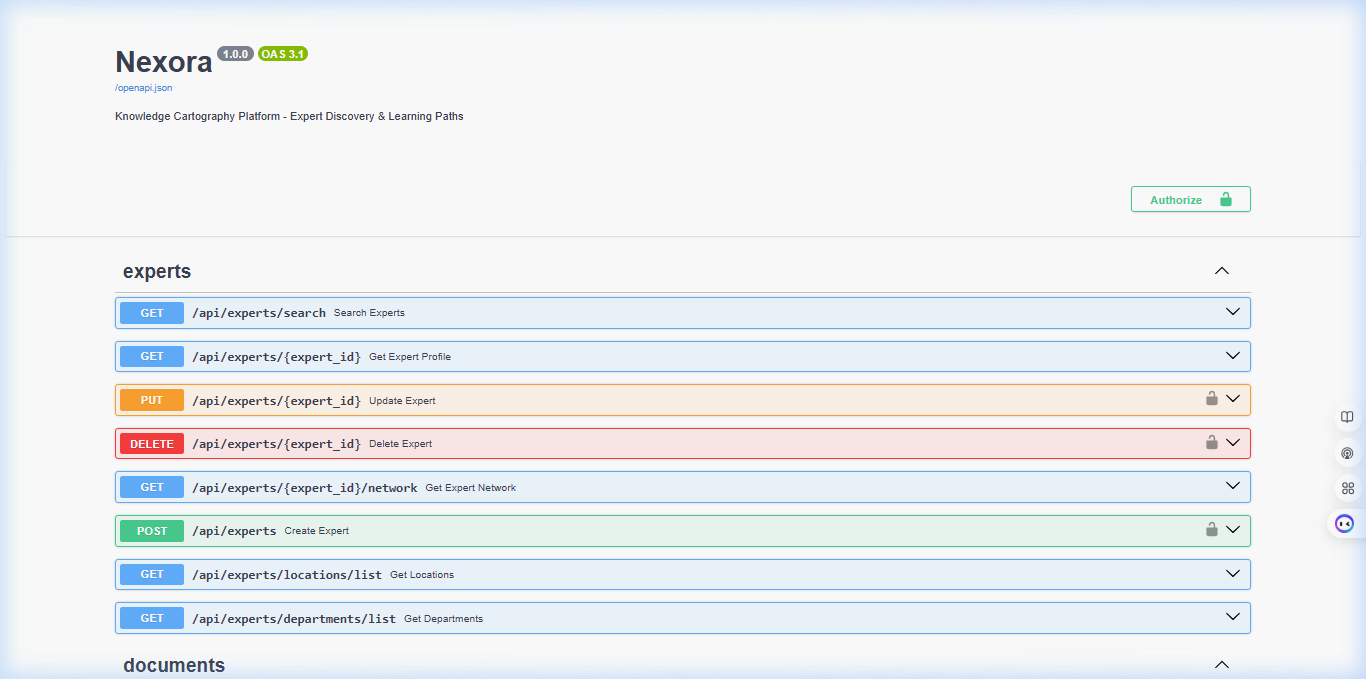
\includegraphics[width=0.95\textwidth]{screenshots/screenshot_swagger.png}
\caption{Documentation interactive de l'API (Swagger / OpenAPI)}
\label{fig:swagger}
\end{figure}

La Figure \ref{fig:swagger} montre la documentation générée automatiquement par OpenAPI. Elle permet de valider rapidement les contrats d'API, de tester les endpoints (auth, IA, Big Data) et de faciliter l'intégration frontend grâce à une référence unique et versionnée.

La documentation Swagger fournit :
\begin{itemize}
  \item \textbf{Liste des endpoints} : tous les routes disponibles organisées par tag
  \item \textbf{Schémas de requête} : structures JSON attendues pour chaque endpoint
  \item \textbf{Schémas de réponse} : structures JSON retournées par chaque endpoint
  \item \textbf{Interface de test} : possibilité d'exécuter des requêtes directement depuis le navigateur
  \item \textbf{Exemples d'utilisation} : exemples concrets pour chaque endpoint
\end{itemize}

\begin{figure}[H]
\centering
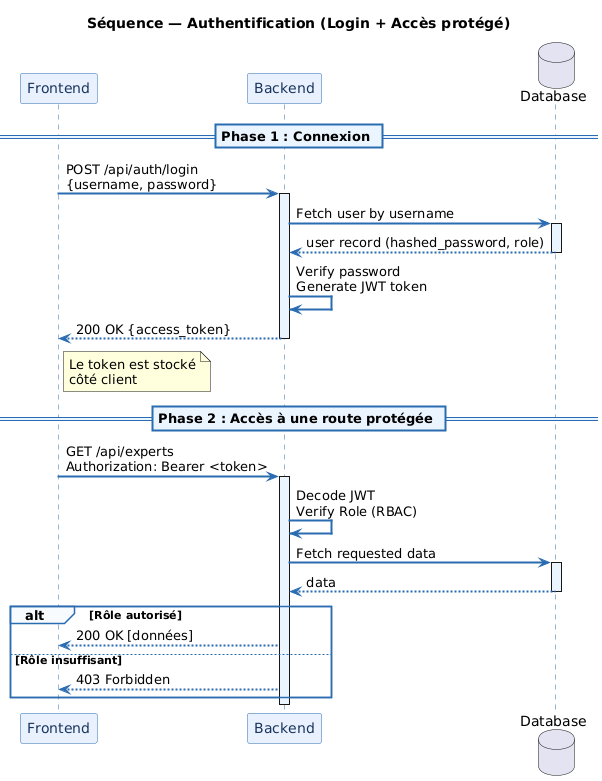
\includegraphics[width=0.95\textwidth]{screenshots/03_sequence_auth.png}
\caption{Séquence d'authentification : login, génération et validation JWT}
\label{fig:seq_auth}
\end{figure}

La Figure \ref{fig:seq_auth} explicite le flux d'authentification : soumission des identifiants, vérification, génération du JWT et réutilisation du token dans l'en-tête \texttt{Authorization}. Ce flux est central pour appliquer le RBAC et protéger les endpoints sensibles.

Les étapes du flux d'authentification sont :
\begin{itemize}
  \item \textbf{Soumission} : l'utilisateur envoie email et mot de passe via le formulaire
  \item \textbf{Vérification} : le backend vérifie les identifiants contre la base de données
  \item \textbf{Génération JWT} : si valide, un token JWT est généré avec claims (sub, role, exp)
  \item \textbf{Stockage} : le token est stocké côté client (localStorage)
  \item \textbf{Utilisation} : le token est transmis dans l'en-tête Authorization pour les requêtes API
  \item \textbf{Validation} : chaque endpoint valide le token avant d'exécuter la logique métier
\end{itemize}

\section{Endpoints API}
\begin{table}[H]
\centering
\caption{Endpoints d'authentification}
\label{tab:auth_endpoints}
\begin{tabular}{p{4.5cm} p{2.2cm} p{7cm}}
\toprule
\textbf{Endpoint} & \textbf{Méthode} & \textbf{Description} \\
\midrule
/api/auth/register & POST & Inscription avec validation Pydantic \\
/api/auth/login & POST & Login JSON + rate limiting \\
/api/auth/verify & GET & Vérification token \\
/api/auth/me & GET & Profil courant à partir du JWT \\
\bottomrule
\end{tabular}
\end{table}

Ces endpoints constituent la base de la sécurité applicative : \texttt{/login} délivre un token signé, \texttt{/verify} valide sa conformité, et \texttt{/me} permet au frontend de récupérer le profil courant sans stocker d'état côté serveur. La présence d'une documentation interactive (Swagger) accélère le test manuel et réduit les erreurs d'intégration : chaque champ attendu et chaque code de retour sont explicités.

L'endpoint \texttt{/api/auth/register} permet la création de nouveaux comptes utilisateur avec une validation stricte des données d'entrée via Pydantic. Les champs obligatoires incluent l'email (vérifié pour l'unicité), le mot de passe (hashé avec bcrypt avant stockage), le nom et le rôle par défaut. Cette validation côté serveur empêche l'injection de données malveillantes et garantit l'intégrité de la base d'utilisateurs dès l'inscription.

L'endpoint \texttt{/api/auth/login} implémente un mécanisme de rate limiting pour prévenir les attaques par force brute. Après un nombre prédéfini de tentatives échouées depuis la même adresse IP, l'endpoint retourne une erreur 429 (Too Many Requests) pendant une période de refroidissement. Cette protection est essentielle pour sécuriser le point d'entrée principal du système et protéger les comptes utilisateur contre les tentatives d'intrusion automatisées.

L'endpoint \texttt{/api/auth/verify} est utilisé par le frontend pour vérifier périodiquement la validité du JWT stocké côté client. Cette vérification permet de détecter les tokens expirés et de rediriger l'utilisateur vers la page de connexion avant que les requêtes API ne commencent à échouer. Cette approche proactive améliore l'expérience utilisateur en évitant les erreurs inattendues lors de l'utilisation de l'application.

L'endpoint \texttt{/api/auth/me} retourne le profil complet de l'utilisateur authentifié (nom, email, rôle, département, compétences) en extrayant ces informations directement du JWT sans requêter la base de données. Cette optimisation réduit la charge sur la base de données et améliore les performances pour les endpoints qui ont besoin d'afficher les informations utilisateur dans l'interface (par exemple, dans la barre de navigation ou les pages de profil).

\section{Authentification JWT}
L'authentification repose sur JWT afin d'assurer un backend stateless. Le token est généré à la connexion après vérification des identifiants et est signé côté serveur afin d'empêcher toute falsification. Il contient les claims essentiels : \texttt{sub} (identité), \texttt{role} (rôle RBAC) et \texttt{exp} (expiration), ce qui permet au backend de décider rapidement des droits d'accès sans maintenir de session côté serveur.

Le processus de génération du JWT utilise une clé secrète (configurable via variable d'environnement \texttt{SECRET\_KEY}) et l'algorithme de signature HS256. Cette clé doit être gardée confidentielle et ne doit jamais être exposée dans le code source ou les logs. En production, il est recommandé d'utiliser une clé longue et générée aléatoirement, et de la faire circuler via des secrets management (Vault, AWS Secrets Manager, etc.) plutôt que via des variables d'environnement simples.

Le claim \texttt{sub} (subject) contient l'identifiant unique de l'utilisateur (typiquement son email ou son ID dans la base de données). Ce claim est utilisé par les gardes d'autorisation pour identifier l'utilisateur courant et récupérer ses informations supplémentaires si nécessaire. Le claim \texttt{role} contient le rôle RBAC de l'utilisateur (user, manager, ou admin) et est utilisé directement par les dépendances d'autorisation pour déterminer si l'utilisateur a le droit d'accéder à un endpoint spécifique sans requêter la base de données.

Le claim \texttt{exp} (expiration) contient le timestamp d'expiration du token, calculé en ajoutant la durée configurée (30 minutes par défaut) au timestamp actuel. Ce claim est vérifié automatiquement par la bibliothèque de décodage JWT, qui retourne une erreur si le token est expiré. Cette expiration automatique limite la fenêtre d'opportunité pour un attaquant qui aurait intercepté un token valide, et force les utilisateurs à se réauthentifier périodiquement, ce qui améliore la sécurité globale du système.

Dans NEXORA, le frontend transmet ce JWT dans l'en-tête \texttt{Authorization: Bearer <token>} lors des appels API. Les gardes d'autorisation appliquent ensuite le contrôle d'accès (user/manager/admin) en fonction du claim \texttt{role}. En cas de token manquant, expiré ou invalide, l'API renvoie des erreurs adaptées (401/403) afin de conserver un comportement explicite et sécurisé.

Le stockage du JWT côté client s'effectue généralement dans le localStorage du navigateur pour une persistance entre les sessions. Cependant, cette approche présente des risques de sécurité si l'application est vulnérable aux attaques XSS (Cross-Site Scripting). Pour atténuer ce risque, le frontend implémente des mesures de protection : validation stricte des entrées utilisateur, sanitization des données affichées, et utilisation de Content Security Policy (CSP) pour limiter l'exécution de scripts non autorisés. Dans une version de production, il serait préférable d'utiliser des cookies HttpOnly avec l'attribut SameSite pour stocker le token.

Les gardes d'autorisation sont implémentés sous forme de dépendances FastAPI qui sont appliquées aux endpoints sensibles. Le garde \texttt{require\_auth} vérifie simplement que le token est présent et valide, tandis que \texttt{require\_manager} vérifie en plus que le rôle est manager ou admin, et \texttt{require\_admin} vérifie que le rôle est admin. Ces gardes peuvent être composés : par exemple, un endpoint peut nécessiter \texttt{require\_auth} pour vérifier l'authentification, puis effectuer des vérifications supplémentaires basées sur l'identité de l'utilisateur (par exemple, vérifier qu'un utilisateur ne peut modifier que ses propres données).

La durée d'expiration est configurable et vaut 30 minutes par défaut, ce qui limite la fenêtre d'usage d'un token compromis. Cette approche est complétée par des pratiques de durcissement (hash des mots de passe, limitation de tentatives de login et séparation claire des endpoints publics/privés). Les mots de passe sont hashés avec bcrypt, un algorithme de hachage lent et adapté spécifiquement aux mots de passe, ce qui rend les attaques par force brute ou par dictionnaire extrêmement coûteuses en temps de calcul.

% =========================================================
% CHAPITRE 8 — FRONTEND React
% =========================================================
\newpage
\chapter{Frontend React}

\section{Architecture du Frontend}
Le frontend de NEXORA est une \textbf{SPA} construite avec React 18 et TypeScript. Cette architecture permet une navigation fluide, des composants réutilisables et une modularité adaptée aux nombreux modules fonctionnels.

Le frontend contient \textbf{17 pages principales} (dont Login/Register et une page Forbidden). Certaines pages sont réservées aux rôles élevés via \texttt{ProtectedRoute}.

La structure s'appuie sur un routage centralisé et des composants transverses (navigation, layout, gestion du thème). Le typage TypeScript contribue à la fiabilité des échanges avec l'API (contrats, DTO) et limite les erreurs d'exécution. Sur le plan UX, la cohérence est renforcée par l'utilisation de MUI et par la séparation claire entre pages (fonctionnalités) et composants (réutilisables).

L'utilisation de React 18 apporte des améliorations significatives en termes de performance grâce au mode concurrent et au automatic batching, qui regroupe les mises à jour d'état pour réduire les re-rendus inutiles. Les hooks personnalisés permettent d'encapsuler la logique réutilisable (par exemple, \texttt{useAuth} pour la gestion de l'authentification, \texttt{useApi} pour les appels API, \texttt{useWebSocket} pour les connexions temps réel), ce qui améliore la maintenabilité du code et facilite les tests unitaires.

TypeScript apporte une sécurité typage statique qui détecte les erreurs potentielles dès la phase de développement. Les interfaces TypeScript définissent les contrats avec l'API backend, garantissant que les structures de données sont cohérentes entre le frontend et le backend. Par exemple, l'interface \texttt{User} définit les propriétés attendues pour un utilisateur (id, name, email, role, etc.), et TypeScript vérifie que toutes les utilisations de cette interface respectent ces propriétés, réduisant ainsi les erreurs d'exécution liées à des propriétés manquantes ou mal typées.

Le routing est géré par React Router, qui permet une navigation déclarative et des transitions fluides entre les pages sans rechargement complet du navigateur. Les routes sont protégées par le composant \texttt{ProtectedRoute}, qui vérifie la présence d'un JWT valide et redirige vers la page de connexion si nécessaire. Les routes sensibles (administration, gestion des utilisateurs) utilisent des gardes supplémentaires pour vérifier que l'utilisateur dispose des rôles appropriés (manager ou admin).

\begin{figure}[H]
\centering
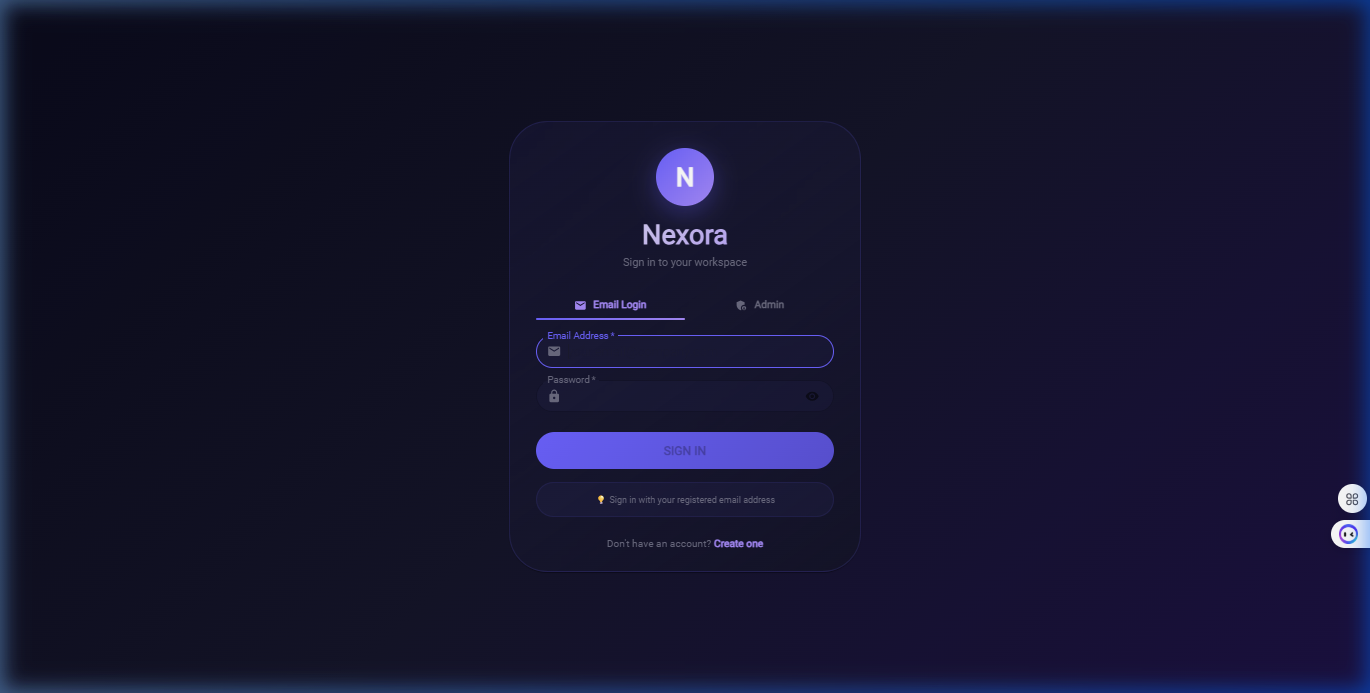
\includegraphics[width=0.85\textwidth]{screenshots/login.png}
\caption{Écran de connexion (frontend)}
\label{fig:login}
\end{figure}

La Figure \ref{fig:login} illustre l'entrée du système. Une fois l'utilisateur authentifié, le JWT est stocké côté client et utilisé pour accéder aux pages protégées et aux fonctionnalités (graphe, recherche, IA, collaboration) conformément au rôle.

L'écran de connexion comprend :
\begin{itemize}
  \item \textbf{Formulaire d'authentification} : champs email et mot de passe sécurisés
  \item \textbf{Validation} : vérification du format email et mot de passe minimum
  \item \textbf{Messages d'erreur} : affichage clair en cas d'échec d'authentification
  \item \textbf{Bouton de connexion} : déclenche la requête d'authentification
  \item \textbf{Liens utiles} : option d'inscription ou récupération de mot de passe
\end{itemize}

\section{Visualisation 3D}
La visualisation 3D, basée sur \texttt{react-force-graph-3d}, constitue un élément différenciant de NEXORA. Elle représente les nœuds et liens du graphe dans un espace interactif, avec des interactions (zoom, rotation, survol) et des filtres.

Cette visualisation vise à rendre tangible la structure relationnelle : l'utilisateur peut naviguer entre experts, compétences, projets et documents, puis comprendre les proximités (voisinages) et les ponts entre communautés. Pour préserver la performance, l'UI privilégie des sous-graphes et des filtres, plutôt qu'un affichage exhaustif. L'objectif n'est pas de visualiser \textbf{tout}, mais de fournir un outil d'exploration guidée et exploitable dans un contexte décisionnel.

La bibliothèque \texttt{react-force-graph-3d} utilise WebGL pour le rendu 3D, ce qui permet d'afficher des milliers de nœuds et liens avec des performances satisfaisantes sur les navigateurs modernes. Les interactions utilisateur (zoom, rotation, pan) sont gérées par la bibliothèque et permettent une navigation intuitive dans l'espace 3D. Les nœuds sont colorés selon leur type (experts en bleu, compétences en vert, projets en orange, documents en violet) et leur taille peut varier en fonction de métriques comme le degré de centralité ou le nombre de connexions.

Les filtres permettent à l'utilisateur de restreindre l'affichage à un sous-graphe pertinent : par exemple, filtrer par département pour visualiser uniquement les experts d'un service, ou filtrer par compétence pour identifier les experts possédant une compétence spécifique. Ces filtres sont appliqués côté backend via des requêtes Cypher optimisées, ce qui réduit la quantité de données transférées et améliore les performances. L'utilisateur peut également sélectionner un nœud spécifique pour afficher ses détails (nom, compétences, projets associés) dans un panneau latéral, ce qui facilite l'exploration contextuelle.

La visualisation 3D est particulièrement utile pour identifier des patterns organisationnels invisibles dans les vues tabulaires traditionnelles : par exemple, on peut repérer des experts qui font le pont entre différents départements (connecteurs), des compétences émergentes qui sont demandées dans plusieurs projets, ou des communautés de pratique regroupées autour de thématiques spécifiques. Ces insights peuvent guider les décisions RH en matière de formation, de mobilité interne ou de constitution d'équipes pluridisciplinaires.

\begin{figure}[H]
\centering
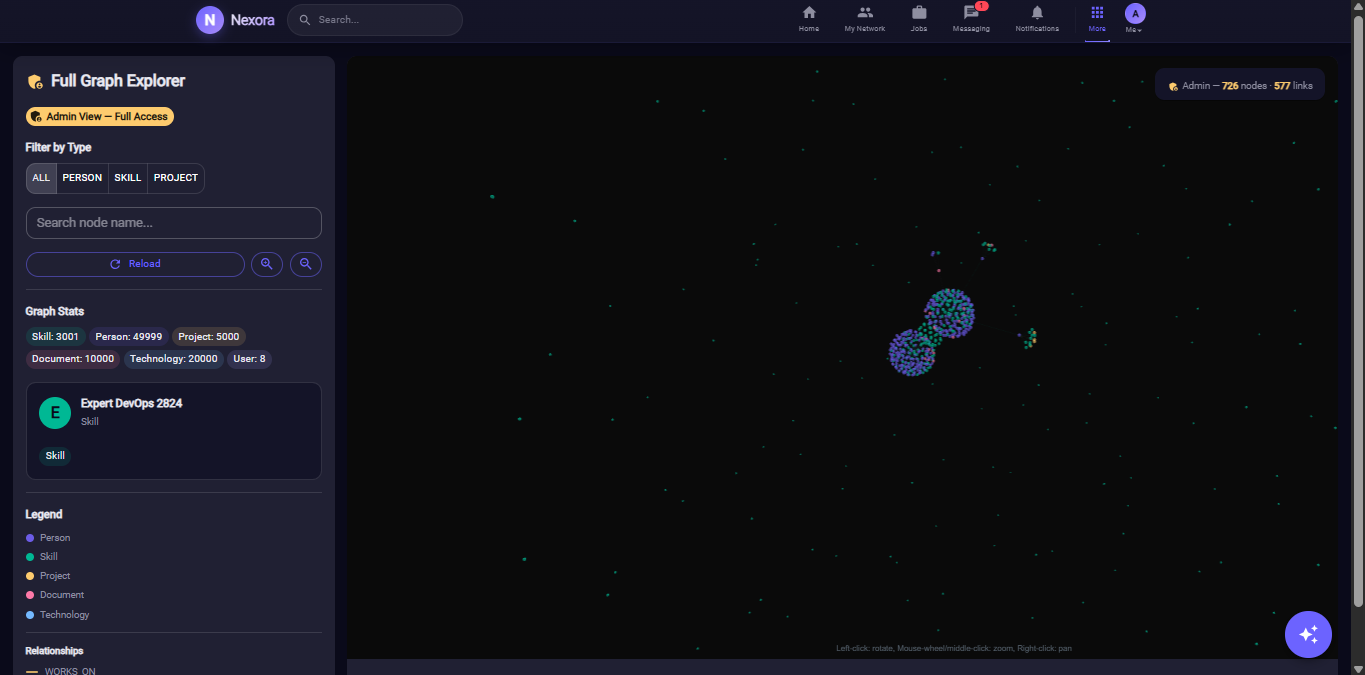
\includegraphics[width=0.95\textwidth]{screenshots/graph.png}
\caption{Visualisation 3D du graphe (interface)}
\label{fig:graph_ui}
\end{figure}

La Figure \ref{fig:graph_ui} met en évidence l'exploration interactive : navigation 3D, sélection de nœuds, affichage contextuel et filtrage. Cette vue est conçue pour rendre la connaissance organisationnelle lisible et exploitable par un utilisateur non technique.

Les fonctionnalités de la visualisation 3D incluent :
\begin{itemize}
  \item \textbf{Navigation 3D} : zoom, rotation, pan pour explorer le graphe
  \item \textbf{Sélection de nœuds} : clic pour afficher les détails d'un expert/compétence/projet
  \item \textbf{Filtrage} : filtres par département, compétence, type de nœud
  \item \textbf{Coloration} : codes couleur par type d'entité pour une lecture rapide
  \item \textbf{Taille dynamique} : taille des nœuds basée sur la centralité ou le degré
  \item \textbf{Légende interactive} : affichage des types et légende du graphe
\end{itemize}

% =========================================================
% CHAPITRE 9 — FONCTIONNALITÉS DE L'APPLICATION
% =========================================================
\newpage
\addtocontents{toc}{\protect\Needspace{6\baselineskip}}
\chapter{Fonctionnalités de l'Application}

\section{Page de Connexion}
La page de connexion constitue la porte d'entrée du système et matérialise l'application du contrôle d'accès. L'utilisateur saisit un identifiant et un mot de passe, puis l'API valide les informations, applique le rate limiting si nécessaire et renvoie un JWT.

\begin{figure}[H]
\centering
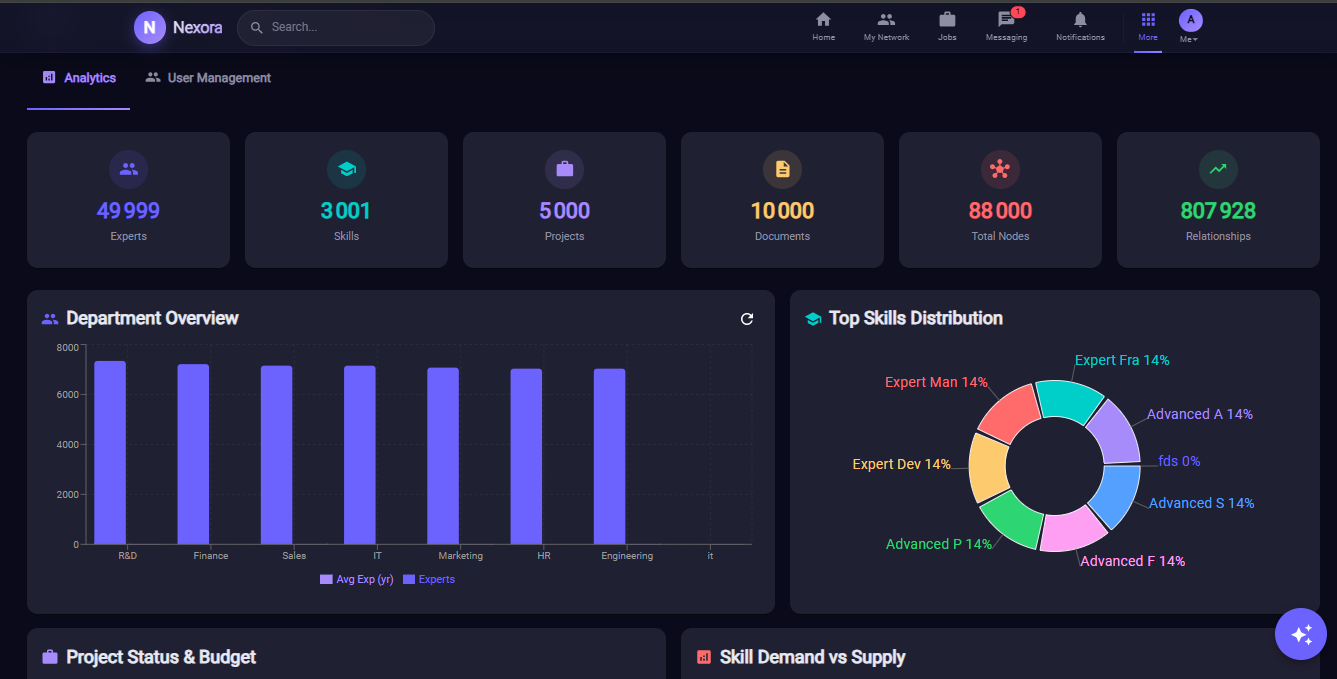
\includegraphics[width=0.95\textwidth]{screenshots/dashboard_1.png}
\caption{Tableau de bord (exemple de visualisation des indicateurs)}
\label{fig:dashboard1}
\end{figure}

La Figure \ref{fig:dashboard1} présente des indicateurs synthétiques (activité, tendances, répartitions) destinés à donner une lecture rapide de l'état du système. Ces visualisations exploitent les endpoints backend et, lorsque nécessaire, les sorties Big Data.

Le dashboard principal affiche :
\begin{itemize}
  \item \textbf{Statistiques générales} : nombre total d'experts, compétences, projets, documents
  \item \textbf{Graphiques d'activité} : activité récente, tendances d'utilisation
  \item \textbf{Répartitions} : distribution par département, par compétence, par rôle
  \item \textbf{Alertes} : notifications d'événements importants ou anomalies
  \item \textbf{Accès rapides} : raccourcis vers les fonctionnalités principales
\end{itemize}

\section{Recherche d'Experts}
La recherche d'experts s'appuie sur un moteur sémantique (TF-IDF + similarité cosinus) exposé par \texttt{POST /api/ai/recommend-experts}. L'approche consiste à représenter le contenu textuel sous forme de vecteurs, puis à classer les experts par score de similarité.

\begin{figure}[H]
\centering
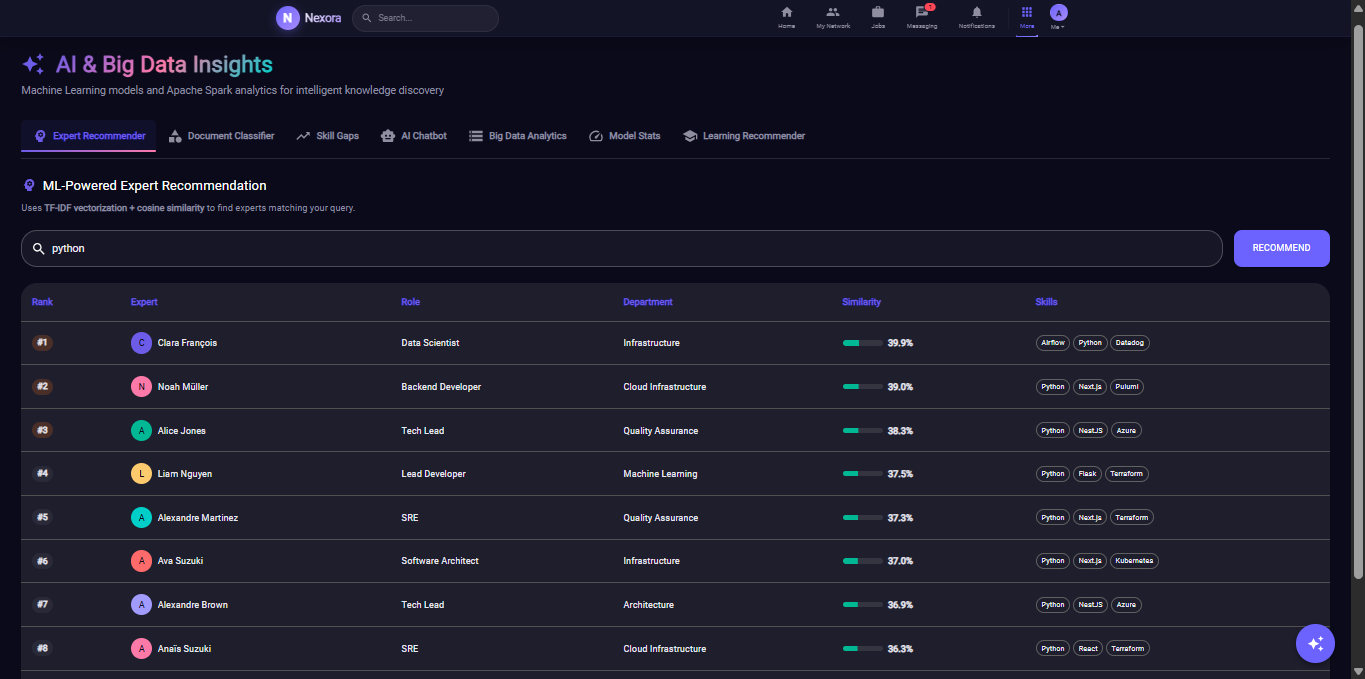
\includegraphics[width=0.95\textwidth]{screenshots/Expert_rec.png}
\caption{Exemple d'interface : recommandation d'experts}
\label{fig:expert_rec}
\end{figure}

La Figure \ref{fig:expert_rec} montre la restitution côté UI d'une recommandation d'experts. Les résultats sont produits à partir de signaux sémantiques et relationnels, puis présentés avec des éléments d'explication (scores, correspondances) afin de justifier le classement.

L'interface de recommandation d'experts comprend :
\begin{itemize}
  \item \textbf{Barre de recherche} : champ de saisie pour la requête en langage naturel
  \item \textbf{Filtres} : filtres par département, compétence, disponibilité
  \item \textbf{Liste de résultats} : experts classés par score de pertinence
  \item \textbf{Détails de chaque expert} : nom, compétences, projets, score de similarité
  \item \textbf{Explication du score} : correspondances avec la requête, facteurs de ranking
  \item \textbf{Actions rapides} : contacter, voir le profil, ajouter aux favoris
\end{itemize}

\Needspace{18\baselineskip}
\section{Chatbot Veda}
Veda constitue un assistant conversationnel intégré, exposé via \texttt{POST /api/ai/chatbot}. L'architecture est \textbf{LLM-first} : si la clé Groq est présente, le backend interroge le modèle ; en l'absence de clé ou en cas d'erreur, le système bascule sur un moteur rule-based.

\begin{figure}[H]
\centering
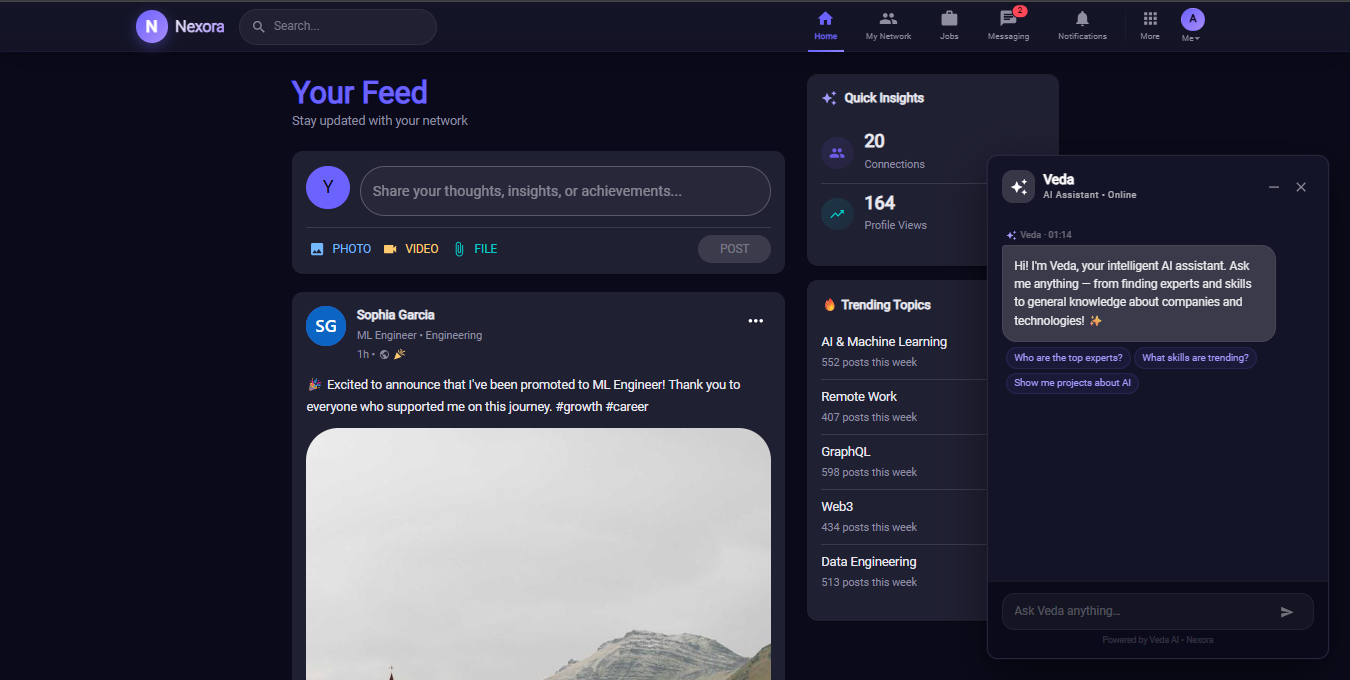
\includegraphics[width=0.85\textwidth]{screenshots/chatboot.png}
\caption{Interface du chatbot Veda}
\label{fig:veda_ui}
\end{figure}

La Figure \ref{fig:veda_ui} illustre l'expérience conversationnelle. Le chatbot fournit un accès naturel à la connaissance interne ; en cas d'indisponibilité du LLM, le backend applique un repli afin de maintenir une réponse utilisable.

L'interface du chatbot Veda inclut :
\begin{itemize}
  \item \textbf{Zone de conversation} : historique des échanges utilisateur/chatbot
  \item \textbf{Champ de saisie} : zone de texte pour poser des questions
  \item \textbf{Indicateur de statut} : affichage du mode (LLM ou rule-based)
  \item \textbf{Suggestions} : questions suggérées pour guider l'utilisateur
  \item \textbf{Formatage des réponses} : réponses structurées avec listes, tableaux si nécessaire
  \item \textbf{Historique} : conservation de l'historique de conversation
\end{itemize}

\begin{figure}[H]
\centering
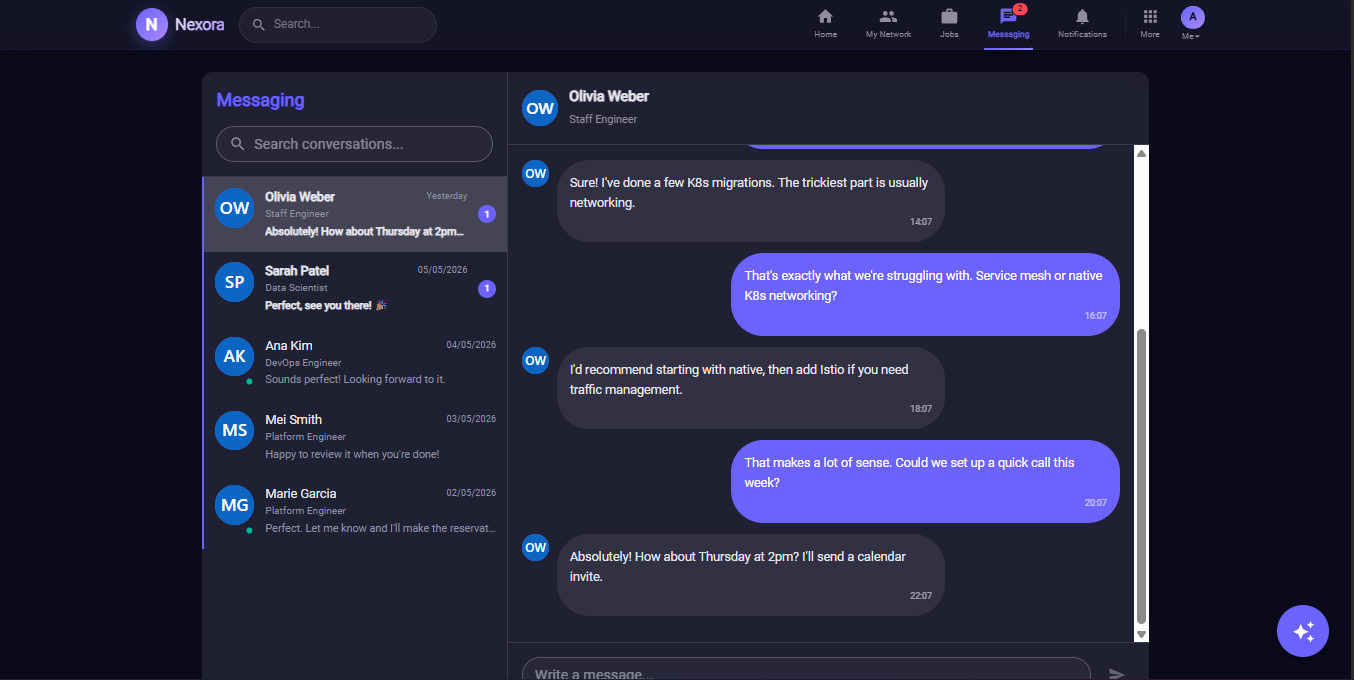
\includegraphics[width=0.95\textwidth]{screenshots/messages.png}
\caption{Messagerie temps réel : échanges et indicateur de saisie}
\label{fig:messaging}
\end{figure}

La Figure \ref{fig:messaging} présente la messagerie, basée sur WebSocket. Elle matérialise les interactions collaboratives (échanges directs, signaux de saisie) et démontre le caractère temps réel de la plateforme.

Les fonctionnalités de messagerie incluent :
\begin{itemize}
  \item \textbf{Communication temps réel} : échanges instantanés via WebSocket
  \item \textbf{Indicateur de saisie} : affichage quand l'autre utilisateur est en train d'écrire
  \item \textbf{Historique} : conservation de l'historique des conversations
  \item \textbf{Notifications} : alertes pour nouveaux messages
  \item \textbf{Groupes} : conversations de groupe pour les équipes ou projets
  \item \textbf{Fichiers} : possibilité d'envoyer des fichiers et documents
\end{itemize}

\begin{figure}[H]
\centering
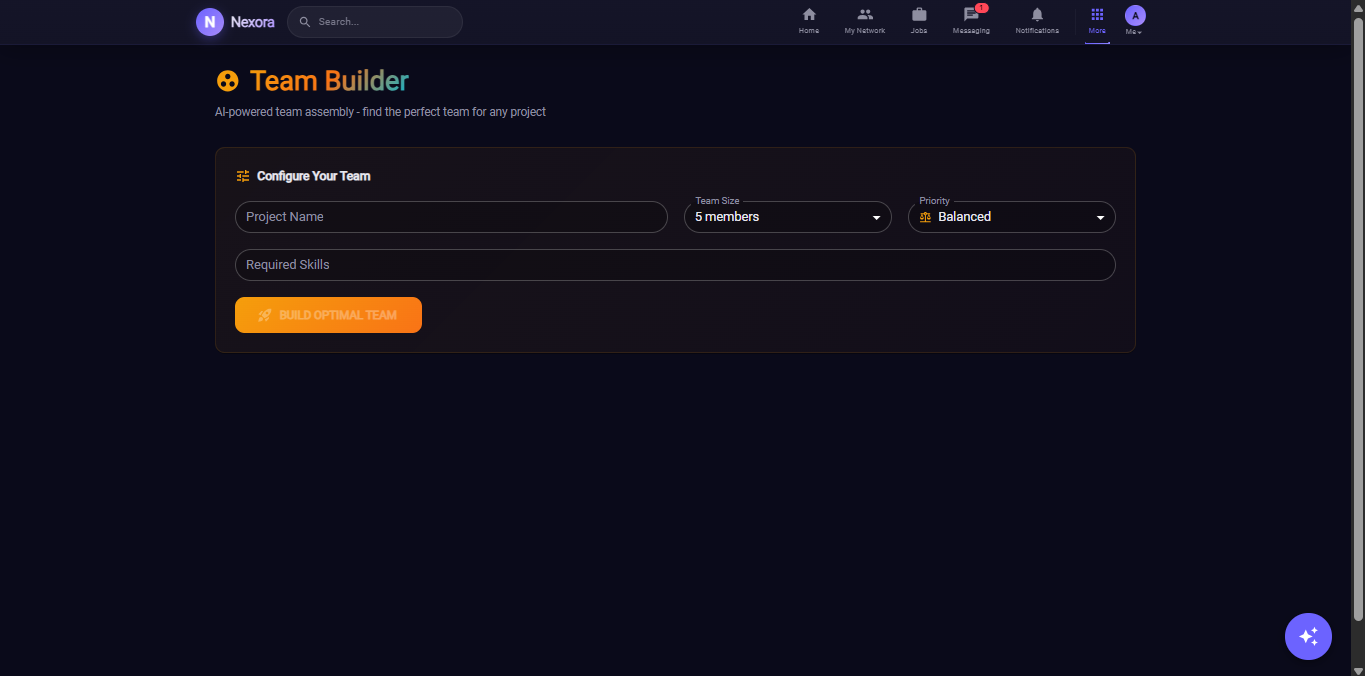
\includegraphics[width=0.95\textwidth]{screenshots/team_builder.png}
\caption{Team Builder : constitution d'équipe orientée compétences}
\label{fig:team_builder}
\end{figure}

La Figure \ref{fig:team_builder} montre un cas d'usage orienté staffing : proposer une équipe à partir d'un besoin, en reliant compétences requises, disponibilité et pertinence des profils. Cette fonctionnalité s'appuie sur la recherche sémantique et les relations du graphe.

Le Team Builder permet de :
\begin{itemize}
  \item \textbf{Définir les besoins} : spécifier les compétences requises pour un projet
  \item \textbf{Rechercher des candidats} : trouver des experts correspondant aux besoins
  \item \textbf{Évaluer la pertinence} : scores de correspondance basés sur compétences et disponibilité
  \item \textbf{Constituer l'équipe} : sélectionner les membres proposés
  \item \textbf{Vérifier l'équilibre} : analyser la composition de l'équipe (compétences, rôles)
  \item \textbf{Exporter} : générer une proposition d'équipe pour validation
\end{itemize}

\begin{figure}[H]
\centering
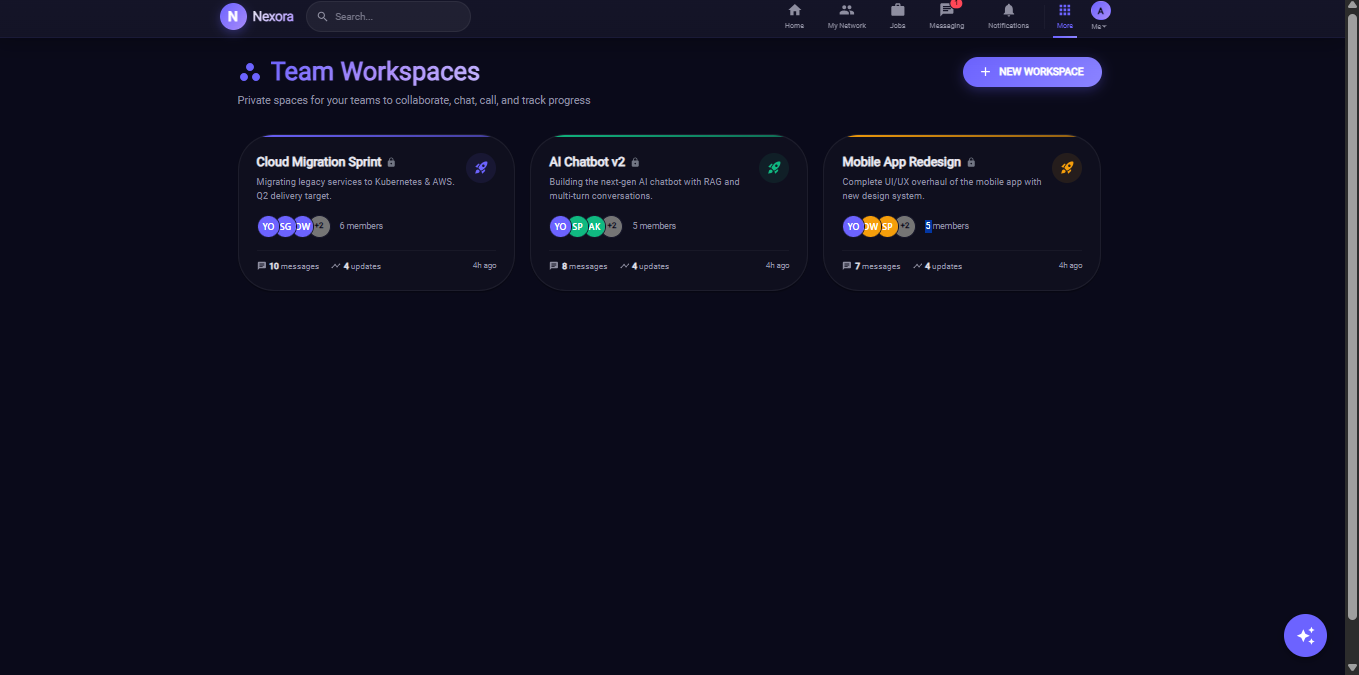
\includegraphics[width=0.95\textwidth]{screenshots/team_workspace.png}
\caption{Workspace d'équipe : collaboration et organisation par projet}
\label{fig:team_workspace}
\end{figure}

La Figure \ref{fig:team_workspace} illustre l'espace de travail partagé : centralisation des échanges, coordination, et support de l'activité projet. L'objectif est de lier le contexte collaboratif aux entités du graphe (projet, membres, compétences).

Les fonctionnalités du workspace d'équipe incluent :
\begin{itemize}
  \item \textbf{Vue de projet} : informations sur le projet, objectifs et livrables
  \item \textbf{Liste des membres} : équipe assignée avec rôles et responsabilités
  \item \textbf{Compétences requises} : compétences nécessaires pour le projet
  \item \textbf{Messagerie de groupe} : canal de communication dédié à l'équipe
  \item \textbf{Suivi de tâches} : gestion des tâches et leur statut
  \item \textbf{Documents partagés} : accès aux documents liés au projet
\end{itemize}

% =========================================================
% CHAPITRE 10 — GUIDE D'INSTALLATION
% =========================================================
\newpage
\chapter{Guide d'Installation}

\section{Prérequis}
L'installation de NEXORA repose prioritairement sur Docker. Configuration minimale : 4 Go RAM (recommandée : 8 Go). Ports requis : 3000 (frontend), 8000 (API), 7474 et 7687 (Neo4j).

Cette approche réduit fortement la complexité d'installation : l'utilisateur n'a pas besoin d'installer manuellement Neo4j, Node.js ou un environnement Python complet. Les services sont isolés et démarrent dans un ordre contrôlé grâce aux healthchecks, ce qui limite les erreurs de dépendances. En complément, un fichier \texttt{.env} centralise les paramètres (URI Neo4j, clé JWT, clé Groq) et permet d'adapter rapidement l'environnement.

Le fichier \texttt{docker-compose.yml} définit l'orchestration complète des services. Chaque service est configuré avec son propre réseau Docker pour assurer l'isolation et la sécurité des communications internes. Les volumes partagés permettent de persister les données Neo4j et de faciliter le développement en montant les fichiers source locaux dans les conteneurs. Les healthchecks sont configurés pour vérifier que chaque service est opérationnel avant de démarrer les services dépendants : par exemple, le backend attend que Neo4j réponde correctement aux requêtes de santé avant de s'initialiser, et le frontend attend que le backend soit accessible avant de servir l'application.

L'installation nécessite simplement Docker et Docker Compose installés sur la machine hôte. Une fois ces prérequis satisfaits, l'utilisateur clone le dépôt, configure le fichier \texttt{.env} avec ses propres clés et paramètres, puis exécute \texttt{docker-compose up --build}. Cette commande construit les images Docker (si nécessaire), démarre tous les services dans l'ordre approprié et expose les ports configurés. L'ensemble du processus prend généralement moins de 10 minutes sur une machine moderne disposant d'une connexion internet pour le téléchargement des images de base.

En cas de problème lors du démarrage, les logs de chaque service sont accessibles via \texttt{docker-compose logs <service>}, ce qui facilite le diagnostic. Les erreurs les plus courantes incluent des ports déjà occupés (conflit avec d'autres applications), des permissions insuffisantes sur les volumes partagés, ou des configurations incorrectes dans le fichier \texttt{.env}. Le guide d'installation fournit des solutions pour ces scénarios, ainsi que des commandes de nettoyage (\texttt{docker-compose down -v}) pour réinitialiser l'environnement si nécessaire.

\begin{figure}[H]
\centering
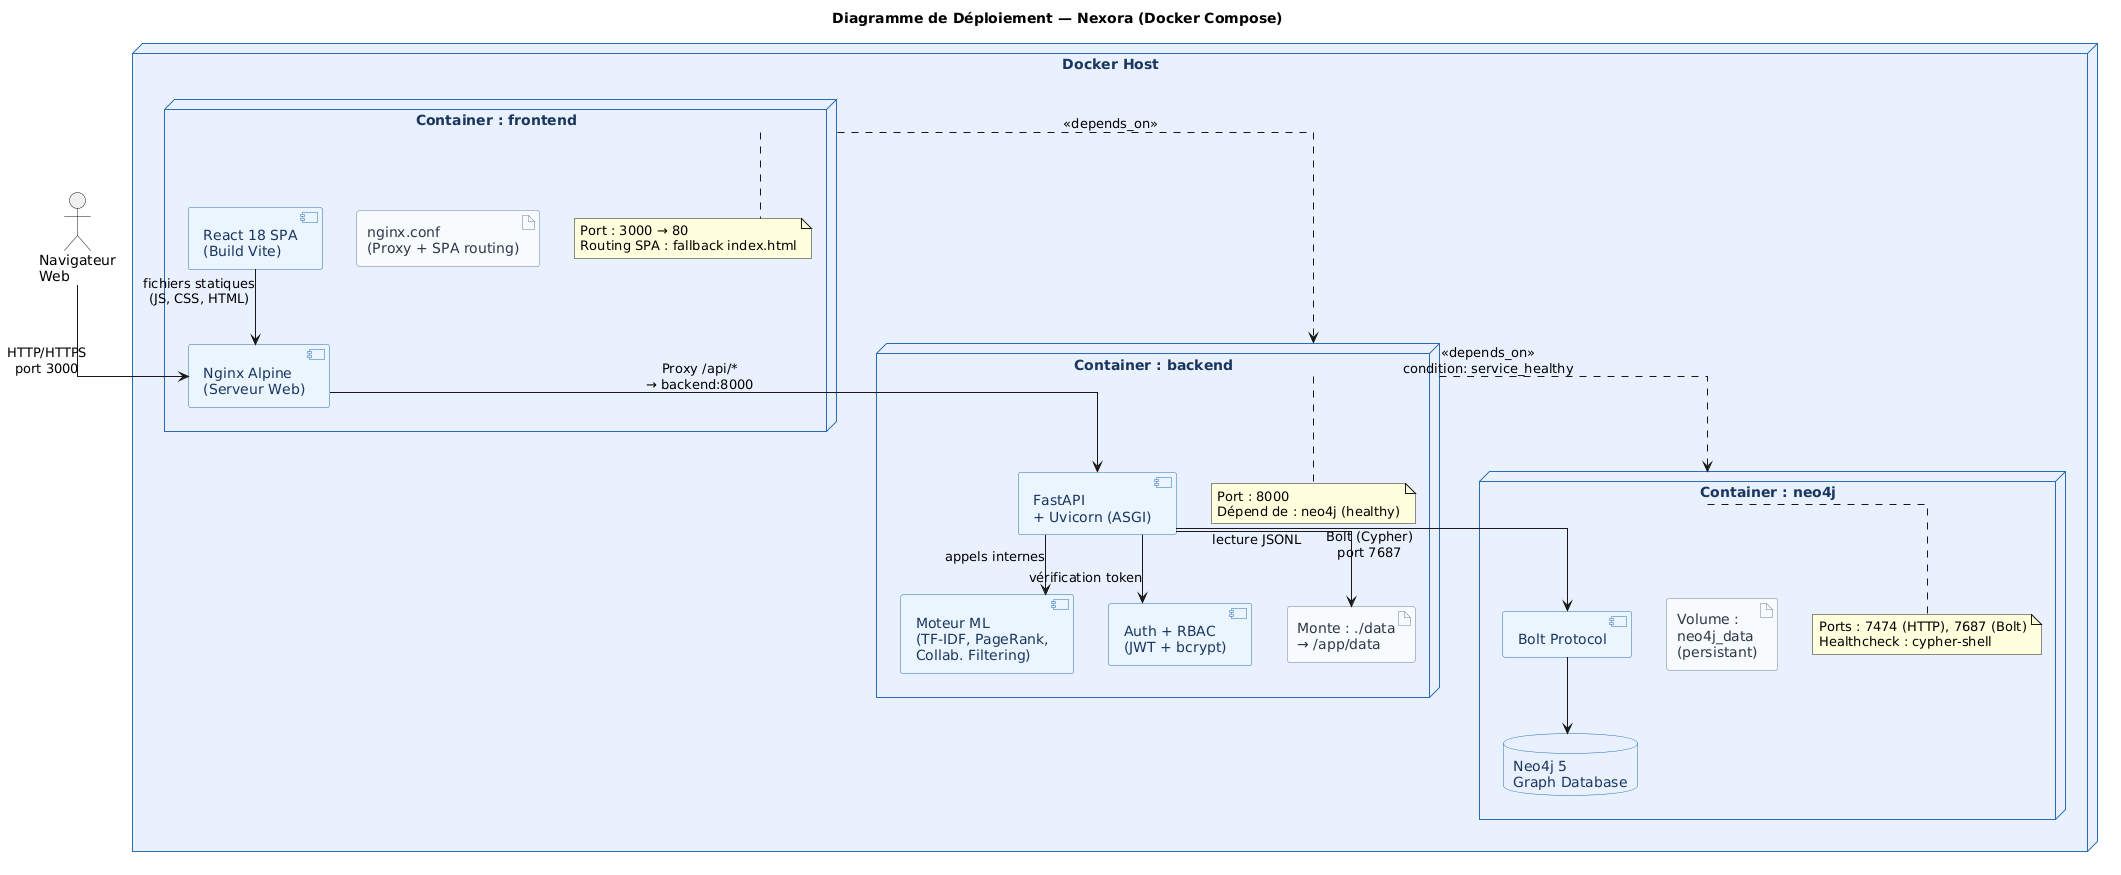
\includegraphics[width=0.95\textwidth]{screenshots/06_deployment.png}
\caption{Schéma de déploiement (Docker Compose / services)}
\label{fig:deployment}
\end{figure}

La Figure \ref{fig:deployment} illustre le déploiement reproductible : services isolés (Neo4j, backend, frontend), healthchecks, ports exposés et orchestration via Docker Compose. Cette approche permet de reproduire l'environnement de démonstration sur une machine neuve avec un minimum de configuration.

L'architecture de déploiement comprend :
\begin{itemize}
  \item \textbf{Service Neo4j} : base de données graphe avec healthcheck
  \item \textbf{Service Backend} : API FastAPI avec dépendances vers Neo4j
  \item \textbf{Service Frontend} : application React servie via Nginx
  \item \textbf{Réseaux Docker} : isolation des communications entre services
  \item \textbf{Volumes} : persistance des données Neo4j et montage des sources
  \item \textbf{Healthchecks} : vérification de santé avant démarrage des dépendants
  \item \textbf{Ports exposés} : 3000 (frontend), 8000 (API), 7474/7687 (Neo4j)
\end{itemize}

\section{Variables d'Environnement}
\begin{table}[H]
\centering
\caption{Variables d'environnement principales}
\label{tab:env_vars}
\begin{tabular}{p{5cm} p{8cm}}
\toprule
\textbf{Variable} & \textbf{Description} \\
\midrule
NEO4J\_URI & URI de connexion Neo4j \\
SECRET\_KEY & Clé secrète de signature JWT \\
ACCESS\_TOKEN\_EXPIRE\_MINUTES & Durée de validité du token (30 min par défaut) \\
GROQ\_API\_KEY & Clé API Groq (Veda LLM) \\
\bottomrule
\end{tabular}
\end{table}

% =========================================================
% CHAPITRE 11 — DONNÉES DU SYSTÈME
% =========================================================
\newpage
\chapter{Données du Système}

\section{Format des Données}
Les données sont fournies au format \textbf{JSONL} (JSON Lines), adapté aux traitements batch PySpark et aux scénarios de streaming.

Le format JSONL offre un compromis efficace entre simplicité et scalabilité : chaque ligne est un objet autonome, ce qui facilite l'ingestion incrémentale, le traitement distribué et le débogage. Dans NEXORA, ce choix permet de partager un jeu de données reproductible (généré avec seed) et de l'utiliser à la fois pour l'alimentation du graphe Neo4j, pour les traitements ML (features textuelles) et pour les agrégations Big Data.

Contrairement au JSON traditionnel qui nécessite de charger l'intégralité du fichier en mémoire pour le parser, le format JSONL permet de traiter les données ligne par ligne (streaming), ce qui est particulièrement adapté pour les jeux de données volumineux. Chaque ligne peut être lue, validée et traitée indépendamment, ce qui facilite le parallélisme et la résilience aux erreurs : si une ligne est corrompue, elle peut être ignorée sans compromettre le traitement du reste du fichier. Cette propriété est essentielle pour les traitements PySpark, qui distribuent le traitement sur plusieurs nœuds et doivent gérer les partitions de manière autonome.

Les fichiers JSONL de NEXORA sont générés par un script Python paramétrable qui accepte différents presets de taille (small, medium, large). Ce script utilise une seed fixe pour garantir la reproductibilité : deux exécutions avec les mêmes paramètres produiront exactement le même jeu de données. Les données sont générées avec des contraintes de cohérence sémantique : par exemple, les compétences assignées aux employés sont choisies en fonction de leur département (un développeur aura plus de chances d'avoir des compétences techniques qu'un commercial), et les projets incluent des employés dont les compétences correspondent aux besoins du projet. Cette cohérence sémantique est cruciale pour que les algorithmes de recommandation produisent des résultats pertinents et que la visualisation du graphe soit interprétable.

Le script de génération de données produit également des fichiers de métadonnées qui documentent les statistiques du jeu de données (nombre d'employés, distribution des compétences, nombre de projets, etc.). Ces métadonnées sont utilisées pour valider que l'ingestion dans Neo4j s'est déroulée correctement et pour fournir des informations contextuelles dans l'interface (par exemple, afficher le nombre total d'experts dans le système). Les fichiers JSONL peuvent également être utilisés pour créer des jeux de données de test spécifiques (par exemple, un jeu de données contenant uniquement des employés du département "Engineering" pour tester des fonctionnalités spécifiques).

\begin{table}[H]
\centering
\caption{Fichiers de données JSONL}
\label{tab:jsonl_files}
\begin{tabular}{p{5cm} p{3cm} p{6cm}}
\toprule
\textbf{Fichier} & \textbf{Type} & \textbf{Description} \\
\midrule
employees.jsonl & RH & Employés, attributs, compétences imbriquées \\
skills.jsonl & Référentiel & Catalogue de compétences \\
projects.jsonl & Projets & Projets, statuts, compétences requises \\
documents.jsonl & Connaissance & Documents, topics, auteurs \\
\bottomrule
\end{tabular}
\end{table}

\Needspace{22\baselineskip}
\begin{figure}[H]
\centering
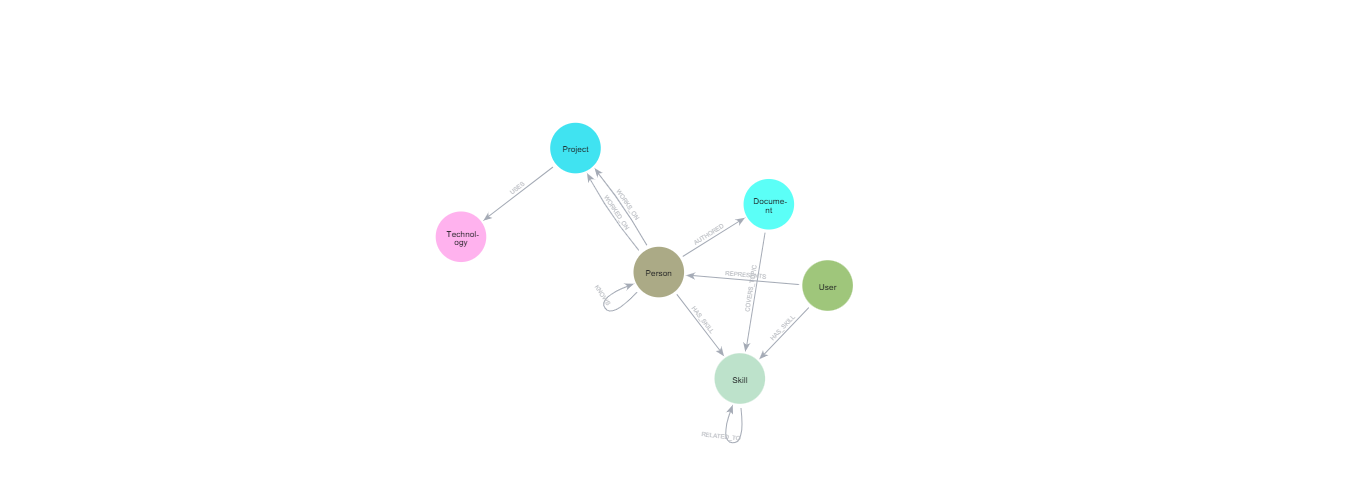
\includegraphics[width=0.95\textwidth]{screenshots/data_model.png}
\caption{Modèle de données (vue applicative et entités principales)}
\label{fig:data_model}
\end{figure}

La Figure \ref{fig:data_model} résume les entités manipulées par la plateforme (experts, compétences, projets, documents) et les relations qui les relient. Cette structuration sert de point de jonction entre les \textbf{fichiers JSONL} (source de données reproductible), l'\textbf{ingestion Neo4j} (modélisation graphe) et la \textbf{couche API} (endpoints de recherche, recommandation et visualisation).

Le modèle de données de NEXORA repose sur :
\begin{itemize}
  \item \textbf{Entités principales} : Employee, Skill, Project, Document, Company, Technology
  \item \textbf{Relations sémantiques} : HAS\_SKILL, WORKS\_ON, CONTRIBUTED\_TO, REQUIRES\_SKILL
  \item \textbf{Attributs riches} : propriétés détaillées pour chaque entité (nom, email, département, etc.)
  \item \textbf{Identifiants stables} : clés uniques garantissant la cohérence entre sources
  \item \textbf{Extensibilité} : possibilité d'ajouter de nouveaux types sans casser l'existant
\end{itemize}

Sur le plan sémantique, le modèle vise à représenter des liens utiles à l'analyse : un expert peut \emph{posséder} ou \emph{maîtriser} des compétences, \emph{participer} à des projets, et \emph{contribuer} à des documents. Ces liens permettent d'exprimer des requêtes Cypher de type « trouver des experts proches d'un besoin », « expliquer une recommandation par un chemin » ou « détecter des ponts inter-départements ».

Les requêtes types supportées par le modèle incluent :
\begin{itemize}
  \item \textbf{Recherche d'experts} : trouver des experts par compétences, projets, département
  \item \textbf{Analyse de centralité} : identifier les experts les plus connectés (PageRank)
  \item \textbf{Détection de communautés} : regrouper les experts par affinités de compétences
  \item \textbf{Ponts inter-départements} : identifier les experts qui connectent différents services
  \item \textbf{Parcours de recommandation} : expliquer une recommandation par un chemin dans le graphe
\end{itemize}

Sur le plan technique, les identifiants et attributs portés par les objets (ex. \texttt{id}, \texttt{department}, \texttt{category}, \texttt{topic}) garantissent la cohérence entre les sources. Les mêmes clés servent :
\begin{itemize}
  \item à charger les données depuis JSONL et à vérifier les correspondances lors de l'ingestion
  \item à indexer les nœuds (pour accélérer la recherche et limiter le coût des traversées)
  \item à alimenter les traitements ML (TF-IDF sur les descriptions/titres, classification par features textuelles, scoring de centralité via PageRank)
  \item à construire des sous-graphes affichables dans la visualisation 3D
\end{itemize}

Cette cohérence technique permet de :
\begin{itemize}
  \item Garantir l'intégrité des données entre JSONL et Neo4j
  \item Optimiser les performances des requêtes Cypher via les index
  \item Faciliter les calculs ML avec des attributs structurés
  \item Assurer une visualisation cohérente et interprétable
\end{itemize}

Enfin, le modèle est conçu pour rester extensible : de nouveaux types (formations, expériences, technologies, certifications) peuvent être ajoutés sans casser les usages existants, à condition de conserver des identifiants stables et des relations explicites. C'est ce choix qui rend possible l'explicabilité : une recommandation n'est pas seulement un score, elle peut être justifiée par des voisinages (compétences partagées), des contextes (projets) et des traces (documents).

Les principes d'extensibilité du modèle sont :
\begin{itemize}
  \item \textbf{Identifiants stables} : les clés ne changent pas pour assurer la continuité
  \item \textbf{Relations explicites} : chaque lien est clairement défini et typé
  \item \textbf{Schéma évolutif} : ajout de nouveaux types sans migration lourde
  \item \textbf{Explicabilité} : chaque recommandation peut être justifiée par un chemin
  \item \textbf{Rétrocompatibilité} : les anciennes requêtes restent valides après extension
\end{itemize}

\begin{figure}[H]
\centering
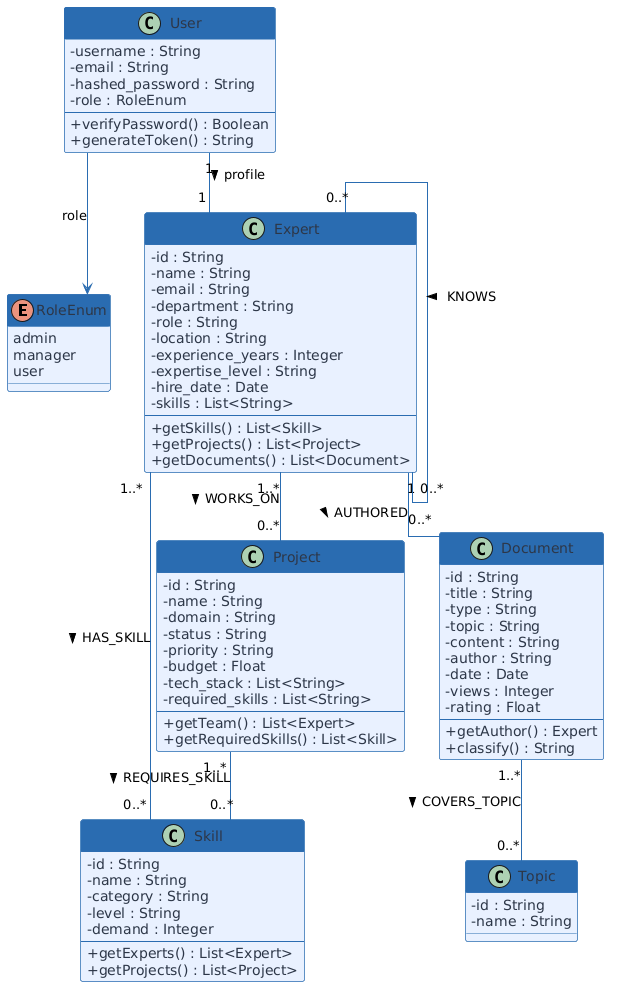
\includegraphics[width=0.95\textwidth]{screenshots/02_class_diagram.png}
\caption{Diagramme de classes (vue de conception)}
\label{fig:class_diagram}
\end{figure}

La Figure \ref{fig:class_diagram} complète la partie données par une vue orientée conception. Elle illustre l'organisation des classes et la séparation entre \textbf{modèles} (structures de données), \textbf{services} (logique métier) et \textbf{couches d'accès} (API / persistance).

L'organisation des classes suit les principes suivants :
\begin{itemize}
  \item \textbf{Modèles Pydantic} : schémas de validation pour entrées/sorties
  \item \textbf{Routeurs FastAPI} : endpoints API organisés par domaine fonctionnel
  \item \textbf{Services métier} : logique métier isolée et réutilisable
  \item \textbf{Accès données} : abstraction pour Neo4j et JSONL
  \item \textbf{Utilitaires} : fonctions partagées (auth, cache, logging)
\end{itemize}

Dans NEXORA, cette séparation est importante pour maintenir l'évolutivité : les modèles Pydantic encadrent les entrées/sorties (validation, sérialisation), les routeurs FastAPI portent les contrats d'API, tandis que les services et utilitaires encapsulent les traitements (scoring, fallback, intégration Groq, calculs Big Data). Concrètement, cette structuration réduit les effets de bord : modifier une règle de sécurité ou une stratégie de recommandation ne nécessite pas de réécrire l'interface utilisateur, et inversement. Le diagramme sert donc de support de compréhension et de maintenance, en particulier lorsqu'on ajoute de nouveaux endpoints ou de nouvelles entités.

Les avantages de cette séparation incluent :
\begin{itemize}
  \item \textbf{Maintenabilité} : chaque couche peut être modifiée indépendamment
  \item \textbf{Testabilité} : tests unitaires isolés par couche
  \item \textbf{Réutilisabilité} : services peuvent être réutilisés dans différents contextes
  \item \textbf{Clarté} : responsabilités claires pour chaque composant
  \item \textbf{Évolutivité} : ajout de nouvelles fonctionnalités sans impact sur l'existant
\end{itemize}

% =========================================================
% CHAPITRE 12 — SÉCURITÉ ET PERFORMANCE
% =========================================================
\newpage
\chapter{Sécurité et Performance}

\section{Authentification et Autorisation}
La sécurité repose sur JWT (stateless) et RBAC. Des gardes centralisées (\texttt{require\_auth}, \texttt{require\_manager}, \texttt{require\_admin}) appliquent les droits. Cette combinaison permet de séparer clairement l'identification (preuve d'identité via le token) et l'autorisation (décision d'accès via le rôle).

Concrètement, les endpoints sensibles imposent une authentification valide, puis vérifient le niveau de privilège requis. Cela se traduit par des réponses explicites (401 si non authentifié, 403 si authentifié mais non autorisé). Côté interface, les pages et actions sont également filtrées pour réduire les erreurs d'usage, mais l'autorité reste le backend : même si un utilisateur manipule l'UI, les gardes empêchent l'accès aux opérations réservées.

La séparation entre identification et autorisation est un principe fondamental de sécurité. L'identification consiste à vérifier que l'utilisateur est bien celui qu'il prétend être (via le JWT), tandis que l'autorisation consiste à vérifier que cet utilisateur a le droit d'effectuer l'action demandée (via le rôle RBAC). Cette séparation permet une gestion fine des permissions : par exemple, un manager peut accéder aux fonctionnalités de staffing (TeamBuilder) mais ne peut pas administrer les utilisateurs, tandis qu'un admin dispose de tous les droits. Les gardes d'autorisation sont appliqués au niveau des endpoints FastAPI, ce qui garantit que toute tentative d'accès non autorisé est bloquée avant même que la logique métier ne soit exécutée.

Le JWT stateless présente l'avantage de ne pas nécessiter de stockage de session côté serveur, ce qui facilite la scalabilité horizontale : plusieurs instances du backend peuvent être déployées derrière un load balancer sans avoir à synchroniser les sessions. Cependant, cela implique que les tokens ne peuvent pas être révoqués facilement avant leur expiration. Pour atténuer ce risque, la durée de vie des tokens est limitée (30 minutes par défaut) et les actions sensibles (suppression de données, modification de rôles) peuvent nécessiter une ré-authentification ou une confirmation supplémentaire. En production, il serait recommandé d'implémenter une liste de révocation (token blacklist) ou d'utiliser des refresh tokens pour améliorer la gestion des sessions.

Les mots de passe sont hashés avec bcrypt avant d'être stockés dans Neo4j. Bcrypt est un algorithme de hachage lent et adapté spécifiquement aux mots de passe : il incorpore un sel (salt) unique pour chaque mot de passe et un facteur de coût (cost factor) qui augmente le temps de calcul nécessaire pour le hachage. Cette caractéristique rend les attaques par force brute ou par dictionnaire extrêmement coûteuses en temps de calcul, ce qui protège les mots de passe même si la base de données est compromise. Le hash bcrypt est vérifié lors de la connexion en comparant le hash stocké avec le hash calculé à partir du mot de passe fourni, sans jamais stocker ni transmettre le mot de passe en clair.

\begin{table}[H]
\centering
\caption{Matrice RBAC (synthèse)}
\label{tab:rbac_matrix}
\begin{tabular}{p{6.5cm} c c c}
\toprule
\textbf{Fonctionnalité} & \textbf{User} & \textbf{Manager} & \textbf{Admin} \\
\midrule
Accès Feed / Profil / Graph / Learning & \checkmark & \checkmark & \checkmark \\
IA (reco, classification, Veda) & \checkmark & \checkmark & \checkmark \\
TeamBuilder (staffing) & & \checkmark & \checkmark \\
Administration utilisateurs & & & \checkmark \\
\bottomrule
\end{tabular}
\end{table}

\begin{figure}[H]
\centering
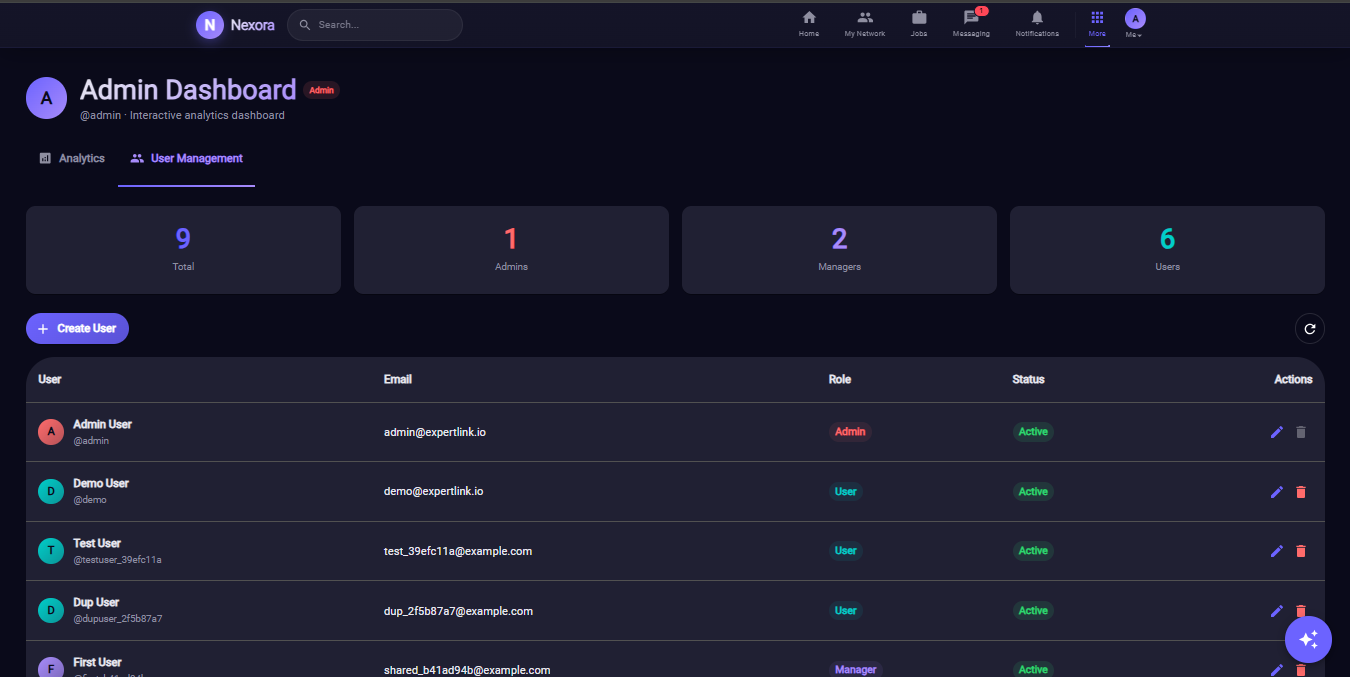
\includegraphics[width=0.95\textwidth]{screenshots/admin_panel.png}
\caption{Administration : gestion des utilisateurs et des rôles (RBAC)}
\label{fig:admin_panel}
\end{figure}

La Figure \ref{fig:admin_panel} illustre l'application du RBAC côté interface : certaines pages et actions (administration, gestion des rôles) ne sont accessibles qu'aux profils autorisés. Le backend applique ces règles via des gardes dédiées.

Le panneau d'administration permet de :
\begin{itemize}
  \item \textbf{Gérer les utilisateurs} : lister, créer, modifier, supprimer des comptes
  \item \textbf{Gérer les rôles} : assigner ou modifier les rôles RBAC (user/manager/admin)
  \item \textbf{Voir les statistiques} : statistiques d'utilisation et d'activité
  \item \textbf{Auditer les actions} : journal des actions sensibles effectuées
  \item \textbf{Configurer le système} : paramètres globaux et configurations
\end{itemize}

\begin{figure}[H]
\centering
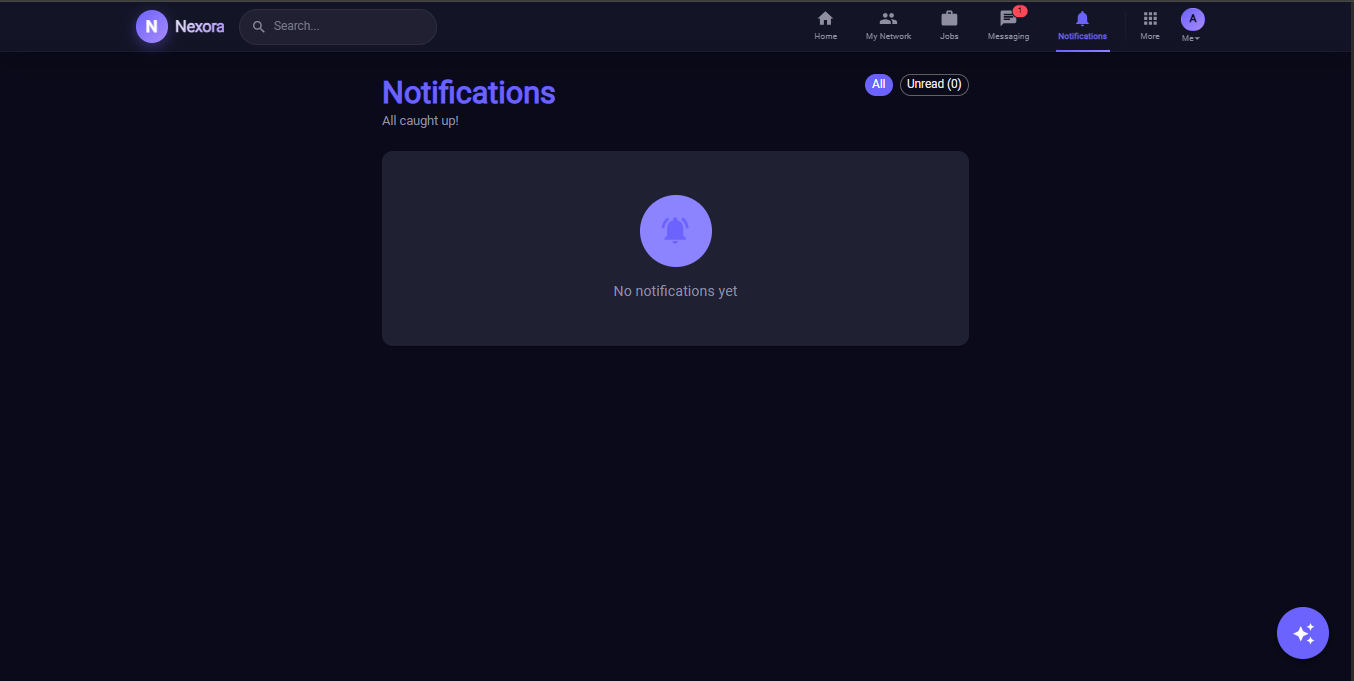
\includegraphics[width=0.95\textwidth]{screenshots/notification.png}
\caption{Notifications : information et suivi d'événements applicatifs}
\label{fig:notifications}
\end{figure}

La Figure \ref{fig:notifications} montre le module de notifications utilisé pour informer l'utilisateur des événements importants (activité, messages, mises à jour). Couplé aux WebSockets, ce composant améliore la réactivité de l'expérience utilisateur.

Le système de notifications inclut :
\begin{itemize}
  \item \textbf{Notifications temps réel} : alertes instantanées via WebSocket
  \item \textbf{Centre de notifications} : historique des notifications consultable
  \item \textbf{Types de notifications} : messages, mentions, mises à jour, alertes système
  \item \textbf{Préférences} : configuration des types de notifications reçues
  \item \textbf{Indicateurs de lecture} : marquage des notifications comme lues/non lues
  \item \textbf{Actions rapides} : possibilité d'agir directement depuis la notification
\end{itemize}

% =========================================================
% CHAPITRE 13 — CONCLUSION ET PERSPECTIVES
% =========================================================
\newpage
\chapter{Conclusion et Perspectives}

\Needspace{10\baselineskip}
\section{Bilan du Projet}
NEXORA a permis de réaliser une plateforme complète combinant backend FastAPI, graphe Neo4j, frontend React moderne et couche IA/Big Data. Le système intègre la recherche sémantique, la classification documentaire, des analyses Spark et un assistant conversationnel (Veda), tout en maintenant une séparation claire des responsabilités (API, données, UI).

Au-delà de l'implémentation fonctionnelle, le projet met en avant une approche orientée \textbf{données et relations} : la connaissance n'est pas seulement stockée, elle est structurée dans un graphe afin de produire des recommandations explicables et des parcours de navigation cohérents. Les choix techniques (JWT/RBAC, conteneurisation, fallback JSONL) ont été intégrés dès la conception pour garantir une solution démontrable, robuste et maintenable.

Le développement de NEXORA a représenté un défi technique significatif, nécessitant l'intégration de technologies diverses et complexes : une base de données orientée graphe (Neo4j), un framework web moderne (FastAPI), une interface utilisateur réactive (React), des algorithmes d'apprentissage automatique (TF-IDF, PageRank, classification), et des outils de traitement de données à grande échelle (PySpark). La coordination de ces technologies dans une architecture cohérente a nécessité une planification rigoureuse, une communication constante au sein du binôme, et une capacité d'adaptation face aux imprévus techniques.

Un aspect particulièrement réussi du projet est la cohérence entre les différentes couches de l'architecture. Le backend expose une API bien documentée via OpenAPI, ce qui a facilité l'intégration avec le frontend. Les modèles de données sont cohérents entre les fichiers JSONL, le schéma Neo4j et les interfaces TypeScript, ce qui a réduit les erreurs d'intégration et facilité le débogage. Les mécanismes de sécurité (JWT, RBAC) sont appliqués de manière cohérente à tous les niveaux, de l'authentification initiale jusqu'aux gardes d'autorisation sur les endpoints sensibles.

La plateforme atteint également un bon équilibre entre fonctionnalité et performance. La visualisation 3D du graphe, bien que techniquement complexe, a été optimisée pour rester responsive grâce à l'utilisation de WebGL et à la limitation de la densité des nœuds affichés. Les algorithmes de recommandation (TF-IDF, PageRank) ont été implémentés avec des mécanismes de cache pour éviter les recalculs inutiles. Le fallback JSONL permet de garantir une continuité de service même lorsque la base de données Neo4j est indisponible, ce qui est essentiel pour les démonstrations et les présentations.

\Needspace{14\baselineskip}
\begin{table}[H]
\centering
\caption{Synthèse des objectifs et état d'implémentation}
\label{tab:objectives_summary}
\begin{tabular}{p{6.5cm} p{7.5cm}}
\toprule
\textbf{Objectif} & \textbf{État observé} \\
\midrule
Cartographie des compétences (graphe 3D) & Visualisation 3D WebGL intégrée \\
Identification d'experts & Endpoint PageRank \\
Recherche sémantique d'experts & TF-IDF + cosinus \\
Big Data (batch) & PySpark + endpoints fallback \\
Sécurité (JWT + RBAC) & Gardes centralisées + expiration configurable \\
\bottomrule
\end{tabular}
\end{table}

\Needspace{10\baselineskip}
\section{Points Forts}
Les points forts ci-dessous synthétisent les apports les plus visibles du projet, autant sur le plan technique (architecture, sécurité, performance) que sur le plan usage (navigation et accès rapide à l'expertise).
\begin{itemize}
  \item \textbf{Graphe de connaissances natif (Neo4j)} : L'utilisation de Neo4j comme base de données principale permet de modéliser explicitement les relations entre entités (experts, compétences, projets, documents). Cette modélisation facilite les requêtes complexes comme la recherche d'experts partageant des compétences, l'identification de ponts entre départements, ou le calcul de centralité via PageRank. Contrairement à une base de données relationnelle qui nécessiterait des jointures complexes et coûteuses, Neo4j permet de traverser les relations de manière native et performante grâce à l'index-free adjacency.

  \item \textbf{Visualisation 3D WebGL} : La visualisation 3D du graphe constitue un élément différenciant de NEXORA. Elle permet aux utilisateurs de naviguer intuitivement dans la structure relationnelle de l'organisation, d'identifier des patterns invisibles dans les vues tabulaires traditionnelles, et de comprendre les proximités entre experts, compétences et projets. L'utilisation de WebGL via la bibliothèque react-force-graph-3d permet d'afficher des milliers de nœuds avec des performances satisfaisantes sur les navigateurs modernes, tout en offrant des interactions riches (zoom, rotation, sélection de nœuds).

  \item \textbf{Approche IA hybride (TF-IDF, classification, PageRank, LLM avec fallback)} : NEXORA combine plusieurs approches d'intelligence artificielle pour offrir des fonctionnalités variées. La recherche sémantique d'experts utilise TF-IDF et la similarité cosinus pour trouver des profils correspondants à des requêtes en langage naturel. La classification documentaire permet d'organiser automatiquement les documents par thématique. Le PageRank identifie les experts les plus centraux dans le graphe organisationnel. L'assistant conversationnel Veda utilise un LLM (Groq) pour offrir un accès naturel à la connaissance, avec un fallback rule-based en cas d'indisponibilité du service externe.

  \item \textbf{Architecture API-First et conteneurisée} : L'architecture API-First de NEXORA garantit que toutes les fonctionnalités sont exposées via des endpoints REST bien documentés (OpenAPI/Swagger). Cette approche facilite l'intégration avec le frontend, permet de tester les endpoints indépendamment, et offre une base solide pour d'éventuelles intégrations avec des systèmes tiers. La conteneurisation via Docker Compose rend l'environnement reproductible et facilite le déploiement : chaque service (Neo4j, backend, frontend) s'exécute dans son propre conteneur avec ses dépendances, et l'orchestration des services est définie de manière déclarative dans le fichier docker-compose.yml.
\end{itemize}

\Needspace{10\baselineskip}
\section{Perspectives d'Amélioration}
Les améliorations envisagées ne remettent pas en cause la complétude du livrable ; elles correspondent à des pistes d'industrialisation et d'enrichissement pour un contexte d'entreprise (volumétrie, supervision, sécurité avancée).
\begin{itemize}
  \item \textbf{Industrialisation du streaming avec Kafka réel} : Le simulateur Kafka actuel démontre le concept de streaming, mais une industrialisation nécessiterait l'intégration d'un cluster Kafka réel pour gérer des flux de données en temps réel à grande échelle. Cela permettrait de capturer les événements organisationnels (nouvelles compétences acquises, nouveaux projets créés, documents publiés) et de les traiter de manière continue pour mettre à jour le graphe de connaissances et les recommandations en temps réel. L'intégration de Kafka nécessiterait également la mise en place de consumers robustes capables de gérer les réordonnements de messages et les pannes de service.

  \item \textbf{Renforcement de GraphRAG} : L'approche GraphRAG (Graph Retrieval-Augmented Generation) pourrait être approfondie pour améliorer les réponses du chatbot Veda. Actuellement, le système utilise une combinaison de requêtes Neo4j et de LLM, mais une implémentation plus sophistiquée pourrait inclure des embeddings de nœuds pour la recherche sémantique dans le graphe, des techniques de résumé de sous-graphes pour contextualiser les requêtes LLM, et des mécanismes de citation des sources pour améliorer l'explicabilité des réponses. Ces améliorations rendraient le chatbot plus précis et plus fiable pour des questions complexes nécessitant une compréhension fine du contexte organisationnel.

  \item \textbf{Amélioration de l'observabilité (métriques, traces)} : Pour un déploiement en production, il serait essentiel d'améliorer l'observabilité du système. Cela inclurait l'intégration d'outils de monitoring comme Prometheus pour collecter des métriques (latence des requêtes, taux d'erreur, utilisation des ressources), Grafana pour visualiser ces métriques en tableaux de bord, et Jaeger ou Zipkin pour le tracing distribué afin de suivre les requêtes à travers les différents services (frontend, backend, Neo4j, Spark). L'ajout de logs structurés et centralisés (via ELK Stack ou Loki) faciliterait le diagnostic des incidents et l'analyse des patterns d'utilisation.

  \item \textbf{Durcissement sécurité (HTTPS, audit logs)} : Bien que NEXORA implémente déjà des mécanismes de sécurité solides (JWT, RBAC, bcrypt), un déploiement en production nécessiterait un durcissement supplémentaire. Cela inclurait l'activation de HTTPS pour toutes les communications (via un reverse proxy Nginx avec TLS), l'implémentation de logs d'audit pour tracer les actions sensibles (modifications de rôles, suppressions de données), l'ajout de mécanismes de rate limiting plus sophistiqués (au-delà du login), et la mise en place de politiques de rotation des secrets (clés JWT, mots de passe). Ces mesures renforceraient la résilience du système contre les attaques et faciliteraient la conformité avec les standards de sécurité d'entreprise.
\end{itemize}

\Needspace{8\baselineskip}
\section{Conclusion Générale}
NEXORA démontre la pertinence d'une approche par graphe pour cartographier les compétences et découvrir l'expertise interne. L'architecture proposée constitue un socle solide pour des évolutions futures vers une plateforme d'intelligence organisationnelle industrialisée.

En conclusion, ce projet a permis de concrétiser une vision ambitieuse : transformer les données RH et organisationnelles en une ressource dynamique et exploitable grâce aux technologies du graphe et de l'intelligence artificielle. La plateforme NEXORA ne se contente pas de stocker des informations sur les employés, leurs compétences et leurs projets ; elle les relie dans un réseau sémantique qui permet de découvrir des insights invisibles dans les systèmes traditionnels : qui sont les experts connecteurs entre les départements, quelles compétences émergentes sont demandées dans les projets, comment constituer des équipes équilibrées pour un nouveau projet.

Le travail réalisé a également permis de valider l'intérêt d'une approche hybride combinant différentes technologies d'IA : les algorithmes classiques (TF-IDF, PageRank) fournissent des résultats déterministes et rapides, tandis que les LLM offrent une flexibilité et une naturalité dans les interactions. L'architecture fallback permet de garantir la continuité de service même lorsque les composants externes sont indisponibles, ce qui est essentiel pour les systèmes critiques en entreprise.

Sur le plan pédagogique, ce projet a été l'occasion de mettre en pratique de nombreux concepts de génie logiciel : architecture en couches, API-First, conteneurisation, tests unitaires, gestion de projet agile, et gestion des risques. La collaboration en binôme a permis de développer des compétences en communication, en coordination technique, et en revue de code. La documentation exhaustive (rapport, guide d'installation, glossaire) garantit que le projet peut être repris et étendu par d'autres développeurs.

Au-delà des aspects techniques, NEXORA illustre comment les technologies modernes (graph databases, LLM, Big Data) peuvent être appliquées à des problématiques concrètes d'entreprise : gestion des talents, constitution d'équipes, partage de connaissances. Dans un monde où les compétences deviennent un actif stratégique, la capacité à cartographier, valoriser et exploiter le capital de connaissances interne devient un avantage compétitif majeur. NEXORA propose une réponse technique à cette problématique, en démontrant qu'il est possible de construire une plateforme complète et fonctionnelle avec des technologies open source et des méthodes de développement agiles.

% =========================================================
% ANNEXES
% =========================================================
\appendix

\newpage
\chapter{Guide de Démarrage Rapide}
\begin{enumerate}
  \item Cloner le dépôt du projet.
  \item Créer un fichier \texttt{.env} avec les variables nécessaires.
  \item Générer les données : \texttt{python data/generate\_data.py --scale large}
  \item Lancer la plateforme : \texttt{docker-compose up --build}
  \item Accéder à l'application : \texttt{http://localhost:3000}
\end{enumerate}

\newpage
\renewcommand{\bibname}{Bibliographie et Webographie}
\addcontentsline{toc}{chapter}{Bibliographie et Webographie}
\begin{thebibliography}{99}
\bibitem{brinpage1998} Sergey Brin and Lawrence Page. The anatomy of a large-scale hypertextual Web search engine. \emph{Computer Networks and ISDN Systems}, 30(1-7):107-117, 1998.
\bibitem{neo4j} Neo4j Documentation. \url{https://neo4j.com/docs/}
\bibitem{fastapi} FastAPI Documentation. \url{https://fastapi.tiangolo.com/}
\bibitem{react} React Documentation. \url{https://react.dev/}
\bibitem{spark} Apache Spark Documentation. \url{https://spark.apache.org/docs/}
\bibitem{groq} Groq Documentation. \url{https://groq.com/docs/}
\end{thebibliography}

\newpage
\chapter{Glossaire}
\begin{longtable}{p{4.5cm} p{10.5cm}}
\toprule
\textbf{Terme} & \textbf{Définition} \\
\midrule
ASGI & Standard Python pour applications web asynchrones \\
Bolt & Protocole de communication utilisé par Neo4j \\
Cypher & Langage déclaratif de requêtes pour Neo4j \\
GraphRAG & Technique combinant graphe de connaissances et LLM \\
JSONL & Format JSON Lines : un objet JSON par ligne \\
JWT & Jeton signé pour authentification stateless \\
LLM & Large Language Model \\
PageRank & Algorithme de centralité dans un graphe \\
RBAC & Contrôle d'accès basé sur les rôles \\
SPA & Single Page Application \\
TF-IDF & Pondération pour représentation textuelle \\
WebGL & API graphique pour rendu 3D dans le navigateur \\
WebSocket & Protocole bidirectionnel pour communication temps réel \\
\bottomrule
\end{longtable}

\end{document}